%\usepackage{amsmath}
%\usepackage{amsfonts}
%\usepackage{amssymb}
%\usepackage{bbm, subfigure, appendix}

%}}}

%{{{ introduction

\chapter{Octree Meshing}
\label{chap:octree}

Spatial decompositions of the $d$-dimensional cube have important
applications in scientific computing: they can be used as algorithmic
foundations for adaptive finite element methods \cite{becker00,kim02},
adaptive mesh refinement methods \cite{griebel98, popinet03}, and
many-body algorithms \cite{greengard89, aluru02, shangHua98, warren92,
ying04, ying03}. The earliest examples of tree-based spatial
decompositions of $\mathcal{R}^n$ can be traced to the use of {\em
binary space partitions} \cite{ fuchs83, fuchs80, schumaker69}.
Binary space partitioning (BSP) is a method for recursively
subdividing a space into convex sets by hyperplanes. This subdivision
gives rise to a representation of the space by means of a tree data
structure known as a BSP tree. The BSP partitions its domain into two
subregions and therefore the BSP tree is a binary tree. BSP trees can
be used in spaces with any number of dimensions, but {\em quadtrees}
\cite{finkel74} and {\em octrees} \cite{meagher82} are most useful in
partitioning 2D and 3D domains, respectively. These use axis aligned
lines and planes, respectively, instead of arbitrary hyperplanes and
are efficient for the specific domains they are intended to work on.

Octrees and quadtrees are usually employed while solving two types of
problems: searching and partitioning. Searches within a domain using
$d$-trees ($d$-dimensional trees with a maximum of $2^d$ children per
node), benefit from the reduction of the complexity of the search from
$\mathcal{O}(n)$ to $\mathcal{O}(\log n)$. Similar benefits can be
obtained by the use of {\em space-filling curves} \cite{tropf81}. This
equivalence has been used in linear quadtree and octree
representations \cite{bern99, tu05}, including the current
work. Unstructured meshes are often preferred over uniform
discretizations because they can be used with complicated domains and
permit rapid grading from small to large elements. However, generating
large unstructured meshes is a challenging task \cite{shewchuk98}. On
the contrary, octree-based unstructured hexahedral meshes can be
constructed efficiently \cite{berti04, greaves99, schneiders97,
schneiders96,shepard91, tu04b}. Although they are not suitable for
highly complicated geometries, they provide a good compromise between
adaptivity and simplicity for numerous applications like solid
modeling \cite{meagher82}, object representation \cite{ayala85,
brunet90}, visualization \cite{freitag99}, image segmentation
\cite{strasters91}, adaptive mesh refinement \cite{griebel98,
popinet03} and N-body simulations \cite{greengard89, aluru02,
shangHua98, warren92, ying04, ying03}.

Octree data structures used in discretizations of partial differential
equations should satisfy certain spatial distribution of octant size
\cite{bern99, tu05}. That is, adjacent octants should not differ
greatly in size\footnote{This is referred to as the 2:1 balance
constraint. A formal definition of this constraint is given in section
\ref{sec:balanceConstraint}.}. Furthermore, conforming discretizations
require a so-called `balance condition' that is necessary to construct
appropriate function spaces.  In particular, when the 2:1 balance
constraint is imposed on octree-based hexahedral meshes, it ensures
that there is at most one {\em dangling} node on any edge or face.
What makes the balance-refinement problem difficult and interesting is
a property known as the {\em ripple effect}: An octant can trigger a
sequence of splits whereby it can force an octant to split, even if it
is not in its immediate neighborhood. Hence, balance-refinement is an
inherently iterative process. Solving the balance-refinement problem
in parallel, introduces further challenges in terms of synchronization
and communication since the ripple can propagate across multiple
processors.

{\em{Related Work.}} Limited work has been done on large scale
parallel construction \cite{ aluru02, warren93, ying03} and balance
refinement \cite{ kim02, tu05} of octrees, and the best known
algorithms exhibit suboptimal isogranular scalability.  The key
component in constructing octrees is the partitioning of the input in
order to achieve good load balancing. The use of space-filling curves
for partitioning data has been quite popular \cite{ aluru02, tu05,
warren93, ying03}. The proximity preserving property of space-filling
curves makes them attractive for data partitioning. All the existing
algorithms for constructing octrees use a top-down approach after the
initial partition. The major hurdle in using a parallel top-down
approach is avoiding overlaps. This typically requires some
synchronization after constructing a portion of the tree \cite{ tu05,
warren93, ying03}. Section \ref{sec:p2o} describes the issues that
arise in using a parallel top-down approach.

Bern et al. \cite{bern99} proposed an algorithm for constructing and
balancing quadtrees for EREW PRAM architectures.  However, it cannot
be easily adapted for distributed architectures. In addition, the
balanced quadtree produced is suboptimal and can have up to 4 times as
many cells as the optimal balanced quadtree. Tu et al.\ \cite{tu05}
propose a more promising approach, which was evaluated on large
octrees. They construct and balance 1.22B octants for the Greater Los
Angeles basin dataset \cite{laData00} on 2000 processors in about 300
seconds. This experiment was performed on the TCS-1 terascale
computing HP AlphaServer Cluster at the Pittsburgh Supercomputing
Center. In contrast, we construct and balance\footnote{While we
enforce the $0$-{\em balance} constraint, \cite{tu05} only enforce the
$1$-{\em balance} constraint. Note that it is harder to $0$-{\em
balance} a given octree. See section \ref{sec:balanceConstraint}
for more details on the different balance constraints.} 1B octants
(approximately) for three different point distributions (Gaussian,
Log-Normal and Uniform) on 1024 processors on the same cluster in
about 60 seconds.

{\em Synopsis and Contributions.} In this paper we present two
parallel algorithms: one to construct complete linear octrees from a
list of points; and one to enforce an optimal 2:1 balance
constraint\footnote{There exists a unique least common balance
refinement for a given octree \cite{moore95}.} on complete linear
octrees.  We use a linear octree Morton-encoding-based representation.
Given a set of points, partitioned across processors, we create a set
of octants that we sort and repartition using the Morton ordering. A
complete linear octree is constructed using the seed octants. Then, we
built an additional auxiliary list of a small number of coarse octants
or {\em blocks}.  This auxiliary octant set encapsulates and
compresses the local spatial distribution of octants; it is used to
accelerate the 2:1-balance refinement, which we implement using a
hybrid strategy: intra-block balancing is performed by a classical
level-by-level balancing/duplicate-removal scheme; and inter-block
balancing is performed by a variant of the ripple-propagation
algorithm proposed in \cite{tu05}.  The main parallel tools used are
sample sorts (accelerated by biotonic sorts), and standard
point-to-point/collective communication calls.\footnote{When we
discuss communication costs we assume a Hypercube network topology
with $\Theta (n_p)$ Bisection Width.}

In a nutshell, the major contributions of this work are:
\begin{itemize}	
	\item A parallel bottom-up algorithm for coarsening octrees,
	which is also used for partitioning the input in our other
	algorithms.
	\item A parallel bottom-up algorithm for constructing linear
	octrees. We avoid the synchronization issues that are usually
	associated with parallel top-down approaches to the problem.
	\item An algorithm for enforcing 2:1 balance refinement in
	parallel. The algorithm constructs the minimum number of nodes to
	satisfy the 2:1 constraint. Its key feature is that it avoids
	parallel searches, which as we show in sections \ref{sec:parBal}
	and \ref{sec:commCost}, are the main hurdles in achieving good
	isogranular scalability.
\end{itemize}

{\em Remark:} The main parallel cost of the algorithm is that related
to the parallel sorts that run in ${\mathcal O}(N \log N)$ work and
${\mathcal O}(\frac{N}{n_p}\, \log(\frac{N}{n_p}) + n_p \log(n_p))$ time, assuming
uniformly distributed points \cite{karypis03}.  In the following
sections we present several algorithms for which we give precise {\tt
work} and {\tt storage} complexity. For some of the parallel
algorithms we also give {\tt time} complexity estimates; this
corresponds to wall-clock time and includes work/per processor and
communication costs. The precise number depends on on the initial
distribution and the effectiveness of the partitioning. Thus the
numbers for {\tt time} are only an estimate under uniform distribution
assumptions. If the {\tt time} complexity is not specifically
mentioned then it is comparable to that of a sample-sort.

{\em{Organization of the paper.}} In section \ref{sec:bg} we introduce
some terminology that will be used in the rest of the paper. Section
\ref{sec:methods} describes the various components of our construction
and balance refinement algorithms. In Section \ref{sec:results} we
present numerical experiments, including fixed size and isogranular
scalability tests on different data distributions. Finally, in Section
\ref{sec:conclude} shortcomings of the proposed approach are discussed
and some suggestions for future work are also offered. Table
\ref{tab:Notations} summarizes the notation that is used in the
subsequent sections.

\begin{table*}
  \centering
  \caption{Notation}
  \begin{tabular}{|ll|} \hline 
    $D_{max}$ & Maximum depth of the tree.\\
    $\mathcal{L}(N)$ & Level of octant $N$.\\		
    $\mathcal{P}(N)$ & Parent of octant $N$.\\
    $\mathcal{S}(N)$ & Siblings (sorted) of octant $N$.\\
    $\mathcal{C}(N)$ & Children (sorted) of octant $N$.\\    								 
    $\mathcal{D}(N)$ & Descendant of octant $N$.\\
    $\mathcal{FC}(N)$ & First child of octant $N$.\\ 				
    $\mathcal{LC}(N)$ & Last child of octant $N$.\\ 				  
    $\mathcal{FD}\left(N,l\right)$ & First descendant of octant $N$ at level $l$.\\
    $\mathcal{LD}\left(N,l\right)$ & Last descendant of octant $N$ at level $l$.\\
    $\mathcal{DFD}(N)$ & Deepest first descendant of octant $N$.\\
    $\mathcal{DLD}(N)$ & Deepest last descendant of octant $N$.\\    
    $\mathcal{A}(N)$ & Ancestor of octant $N$.\\		   
    $\mathcal{A}_{finest}\left(N,K\right)$ & Nearest Common Ancestor of octants $N$ and $K$.\\
    $\mathcal{N}\left(N,l\right)$ & List of all potential neighbors of octant $N$ at level $l$.\\
    $\mathcal{N}^{s}\left(N,l\right)$ & A subset of $\mathcal{N}(N,l)$, with the property that all of\\
    & these share the same common corner with $N$. This \\
    & is also the corner that $N$ shares with its parent.\\
    $\mathcal{N}\left(N\right)$ & Neighbor of $N$ at any level.\\ 
    $\mathcal{I}(N)$ & Insulation layer around octant $N$.\\
    $\{\ldots\}$ & A set of elements.\\           
    $\emptyset$ & The empty set.\\
    $A \leftarrow B$ & Assignment operation.\\
    $A \oplus B$ & Bitwise $A$ {\tt{XOR}} $B$.\\
    $\{A\} ~ \cup ~ \{B\}$ & Union of the sets A and B. The order is\\
    			 						& preserved, if possible.\\
    $\{A\} ~ \cap ~ \{B\}$ & Intersection of the sets A and B.\\    
    $A + B$ & The list formed by concatenating the lists A and B.\\
    $A - B$ & Remove the contents of B from A.\\
    $A[i]$ & $i^{th}$ element in list $A$.\\
    \tt{len}$(A)$ & Number of elements in list $A$.\\
    \tt{Sort}$(A)$ & Sort $A$ in the ascending Morton order.\\
    $A$\tt{.push\_front}$(B)$ & Insert $B$ to the beginning of $A$.\\
    $A$\tt{.push\_back}$(B)$ & Append $B$ to the end of $A$.\\
    $A_{global}$ & Union of the list $A$ from all the processors.\\
    $n_p$ & Total number of processors.\\
    \tt{Send$\left(A\right.$,$r\left.\right)$ } & Send A to processor with rank $ = r$.\\
    \tt{Receive()} & Receive from any processor.\\
    $N_{max}^p$ & Maximum number of points per octant.\\\hline				
 \end{tabular}	
 \label{tab:Notations}	
 \end{table*}

%}}}

%{{{ backround

\section{Background}
\label{sec:bg}
Octrees are trees in which every node has a maximum of eight
children. They are analogous to binary trees (maximum of 2 children
per node) in 1-D and quadtrees (maximum of 4 children per node) in
2-D. A node with no children is called a {\em leaf}. The only node
with no parent is the {\em root}. Nodes that have the same parent are
called {\em siblings}. A node's children, grandchildren and so on and
so forth are collectively referred to as the node's {\em descendants}
and this node will be an {\em ancestor} of its descendants. A node
along with all its descendants can be viewed as a separate tree in
itself with this node as its root. Hence, this set is also referred to
as a {\em subtree} of the original tree. The depth of a node from the
root is referred to as its {\em level}. As shown in
Fig. \ref{fig:octLevels}, the root of the tree is at level 0 and the
children of any node are one level higher than the parent.

\begin{figure}
  \begin{center}
    \subfigure[]{
    \label{fig:octLevels}
    \includegraphics[width=0.3\textwidth]{images/octLevels}}
    %\hspace{.2in}
    \subfigure[]{
    \label{fig:completeOctree}
    \includegraphics[width=0.3\textwidth]{images/linOct}}
    \subfigure[]{
    \label{fig:balancedOctree}
    \includegraphics[height=0.3\textwidth]{images/balOct}}
    \caption{{\tt(a)} Tree representation of a quadtree and {\tt(b)}
    decomposition of a square domain using the quadtree, superimposed
    over an uniform grid, and {\tt(c)} a balanced linear quadtree:
    result of balancing the quadtree.}
  \end{center}
\end{figure}

Octrees and quadtrees\footnote{All the algorithms described in this
paper are applicable to both octrees and quadtrees. For simplicity, we
will use quadtrees to illustrate the concepts in this paper and use
the terms `octrees' and `octants', consistently, in the rest of the
paper.} can be used to partition cuboidal and rectangular regions,
respectively (Fig. \ref{fig:completeOctree}).  These regions are
referred to as the domain of the tree. A set of octants is said to be
complete if the union of the regions spanned by them covers the entire
domain. To reduce storage costs, only the complete list of leaf nodes
is stored, i.e., as a linear octree. To use a linear representation, a
{\em locational code} is needed to identify the octants.  A locational
code is a code that contains information about the position and level
of the octant in the tree. The following section describes one such
locational code known as the {\em Morton encoding}\footnote{Morton
encoding is one of many space-filling curves \cite{zoltan}. Our
algorithms are generic enough to work with other space-filling curves
as well. However, Morton encoding is relatively simpler to implement
since, unlike other space-filling curves, no rotations or reflections
are performed.}.

\subsection{Morton encoding} \label{sec:morton}
 In order to construct a Morton encoding, the maximum possible depth,
$D_{max}$, of the tree is specified {\em a priori}. The domain is
represented by an uniform grid of $2^{D_{max}}$ indivisible cells in
each dimension (Fig. \ref{fig:completeOctree}). Each cell is
identified by an integer triplet representing its $x,y$ and $z$
coordinates, respectively. Any octant in the domain can be uniquely
identified by specifying one of its corners, also known as its anchor,
and its level in the tree (Fig. \ref{fig:mortonInterleaving} ).

\begin{figure}
  \begin{center}
    \includegraphics[width=0.2\textheight]{images/mortonInterleaving}
    \caption{Computing the Morton id of quadrant `d' in the quadtree
    shown in Fig. \ref{fig:completeOctree}. The anchor for any
    quadrant is it's lower left corner.}
    \label{fig:mortonInterleaving}
  \end{center}
\end{figure}

The Morton encoding for any octant is derived by
interleaving\footnote{Instead of bit-interleaving as described here,
we use a multicomponent version (Appendix \ref{app:mortonClass}) of
the Morton encoding scheme.} the binary representations ($D_{max}$
bits each) of the three coordinates of the octant's anchor, and then
appending the binary representation ($(\lfloor(\log_2{D_{max}})\rfloor
+ 1)$ bits) of the octant's level to this sequence of
bits. Interesting properties of the Morton encoding scheme are listed
in Appendix \ref{app:prop}.  In the rest of the paper the terms {\em
lesser} and {\em greater} and the symbols $<$ and $>$ are used to
compare octants based on their Morton ids, and {\em coarser} and {\em
finer} to compare them based on their relative sizes, i.e., their
levels in the octree.

\subsection{Balance Constraint}
\label{sec:balanceConstraint}
In many applications involving octrees, it is desirable that adjacent
elements do not differ greatly in size
\cite{herzen87,kim02,tu05}. Generalizing Moore's \cite{moore95}
categorization of the general balance conditions, we have the
following definition:
\begin{define}
A linear $d$-tree is $k$-balanced if and only if, for any $l \in
[1,D_{max})$, no leaf at level $l$ shares an $m$-dimensional
face\footnote{A corner is a 0-dimensional face, an edge is a
1-dimensional face and a face is a 2-dimensional face.} $\left( m \in
[k,d) \right)$ with another leaf, at level greater than $l+1$.
\end{define}

For the specific case of octrees we use $2$-{\em balanced} to refer to
octrees that are balanced across faces, $1$-{\em balanced} to refer to
octrees that are balanced across edges and faces, and $0$-{\em
balanced} to refer to octrees that are balanced across corners, edges
and faces. An example of a $0$-{\em balanced} quadtree is shown in
Figure \ref{fig:balancedOctree}. The balance algorithm proposed in
this work is capable of $k$-{\em balancing} a given complete linear
octree, and since it is hardest to $0$-{\em balance} a given octree we
report all results for the $0$-{\em balance} case.

%}}}

%{{{ methods

\section{Algorithms}
\label{sec:methods}
\subsection{Constructing large linear octrees in parallel}
\label{sec:p2o}
Octrees are usually constructed by using a top-down approach: starting
with the root octant, cells are split iteratively based on some
criteria, until no further splits are required. This is a simple and
efficient sequential algorithm. However, it's parallel analogue is not
so. We use the case of point datasets to discuss some shortcomings of
a parallel top-down tree construction. Formally, the problem might be
stated as: Construct a complete linear octree in parallel from a
distributed set of points in a domain with the constraint that no
octant should contain more than $(N_{max}^p)$ number of points. Each
processor can independently construct a tree using a top-down approach
on its local set of points.  Constructing a global linear octree
requires a parallel merge. Merging however, is not straightforward.
\begin{enumerate}
\item Consider the case where the local number of points in some
region on every processor was less than $(N_{max}^p)$, and hence all
the processors end up having the same level of coarseness in the
region. However, the total number of points in that region could be
more than $(N_{max}^p)$ and hence the corresponding octant should be
refined further.
\item In most applications, we would also like to associate a unique
processor to each octant. Thus, duplicates across processors must be
removed.
\item For linear octrees overlaps across processors must be resolved.
\item Since there might be overlaps and duplicates, not all the work
done by the processors can be accounted as useful work. This is a
subtle yet important point to consider while analyzing the algorithm
for load-balancing.
\end{enumerate}
Previous work \cite{aluru02, tu05, warren93, ying03} on this problem
has addressed these issues; However, all the existing algorithms
involve many synchronization steps and thus suffer from a sizable
overhead, resulting in suboptimal isogranular scalability. Instead, we
propose a bottom-up approach for constructing octrees from points. The
crux of the algorithm is to distribute the data across the processors
in such a way that there is uniform load distribution across
processors and the subsequent operations to build the octree can be
performed by the processors independently, i.e., requiring no
additional communication.

First, all points are converted into octants at the maximum depth and
then partitioned across the processors using the algorithm described
in Section \ref{sec:blkPart}. This produces a contiguous set of coarse
blocks (with their corresponding points) on each processor. The
complete linear octree is generated by iterating through the blocks
and by splitting them based on number of points per
block\footnote{Refer to the Appendix \ref{app:specialCon} on how to sample
the points in order to construct the coarsest possible octree.}. This
process is continued until no further splits are required. This
procedure is summarized in Algorithm \ref{alg:p2o}.

Next we describe algorithmic components that are fundamental to our
construction and balance refinement algorithms: 1) the generation
of a coarse linear octree between two given octants; 2) generation of
a complete linear octree from a partial set of octants; and 3)
coarsening of octrees.

\begin{table*} 
\centering
\rule{\textwidth}{0.01mm}
\begin{algorithm}{ \textsc{Constructing a complete linear octree from a distributed list of points (parallel)} \tt{- Points2Octree}}
\rule{\textwidth}{0.01mm}
\flushleft
\begin{tabbing}
\tt{\bf{Input:~~~~~~~~}} \= \tt{A distributed list of points, $L$ and a parameter, $(N_{max}^p)$,}\\
 \>\tt{which specifies the maximum number of points per octant.}
\end{tabbing}
\tt{\bf{Output:~~~~~}} Complete linear Octree, $B$.\\
\tt{\bf{Work:~~~~~~~~}} $\mathcal{O}(n\log n),$ where $n = $ len$(L)$.\\
\tt{\bf{Storage:~~~~~}} $\mathcal{O}(n),$ where $n = $ len$(L)$.\\
%\tt{\bf{Time:~~~~~~~~}} ${\mathcal O}(n/n_p\, \log(n/n_p)) +$ Sort/BlockPartition.\\
~\\
1. $F \leftarrow $ [Octant$(p, D_{max}), \forall p \in L ]$\\
2. Sort($F$)\\
3. $B \leftarrow$ BlockPartition($F$) ( Algorithm \ref{alg:blkPart} ) \\
\begin{tabbing}
4. {\bf for} \= \bf{each} $b$ $\in  B$\\
5.   \> {\bf if} \= NumberOfPoints($b$) $> N_{max}^p$\\
6.   \>  \> $B \leftarrow B - b + \mathcal{C}(b)$\\
7.   \> {\bf end if}\\
8. {\bf end for}
\end{tabbing}
 \label{alg:p2o}
\end{algorithm}
\rule{\textwidth}{0.01mm}
\end{table*}

\subsection{Constructing a minimal linear octree between two octants}
\label{sec:compReg}
Given two octants, $a$ and  $b > a$, we wish to generate the minimal number of octants that span the region between $a$ and $b$ according to the Morton ordering. The algorithm (Algorithm \ref{alg:compReg}) first calculates the nearest common ancestor of the octants $a$ and $b$. This octant is split into its eight children. Out of these, only the octants that are either greater than $a$ and lesser than $b$ or ancestors of $a$ are retained and the rest are discarded. The ancestors of either $a$ or $b$ are split again and we iterate until no further splits are necessary. This produces the minimal coarse complete linear octree between the two octants $a$ and $b$. This is illustrated in Figure \ref{fig:compReg}. This algorithm is based on the Properties \ref{prop:decFirst} and \ref{prop:ancLesser} of the Morton ordering, which are listed in Appendix \ref{app:prop}.

\begin{figure}
  \begin{center}
    \includegraphics[angle=90,width=0.9\textwidth]{images/compReg}
    \caption{{\tt(a)} Two cells: Input to {\tt Algorithm \ref{alg:compReg}}. {\tt(b)} The minimal number of octants between the cells given in {\tt(a)}. This is produced by using {\tt(a)} as input to {\tt Algorithm \ref{alg:compReg}}.}
    \label{fig:compReg}
  \end{center}
\end{figure}


\begin{table*}
\centering
\rule{\textwidth}{0.01mm}
\begin{algorithm}{ \textsc{Constructing a minimal linear octree between two octants (sequential)} \tt{- CompleteRegion}}
\rule{\textwidth}{0.01mm}
\flushleft
\tt{\bf{Input:~~~~~~~~}} Two octants, $a$ and  $b > a$.\\
\tt{\bf{Output:~~~~~~}} $R,$ the minimal linear octree between $a$ and $b$.\\
\tt{\bf{Work:~~~~~~~~}} $\mathcal{O}(n\log n),$ where $n = $ len$(R)$.\\
\tt{\bf{Storage:~~~~~}} $\mathcal{O}(n),$ where $n = $ len$(R)$.\\
  ~\\
\begin{tabbing}  
1. {\tt $W \leftarrow  \mathcal{C}(\mathcal{A}_{finest}\left(a,b\right))$}\\
2. \tt{\bf{for}} \= \bf{each} {$w \in W$}\\
3.      \> \tt{\bf {if}} \= \tt{$\left(a < w < b\right)$ AND $\left(w \notin \left\{\mathcal{A}(b)\right\}\right)$}\\
4.      \> \> $R \leftarrow R + w$\\
5.      \> \tt{\bf {else if}} \= {$\left(w \in \left\{\left\{\mathcal{A}(a)\right\},\left\{\mathcal{A}(b)\right\}\right\}\right)$}\\
6.      \> \> $W \leftarrow W - w + \mathcal{C}(w)$\\
7.			\> \tt{\bf{end if}}\\
8. \tt{\bf{end for}}\\
9. Sort(R)
\end{tabbing}
\label{alg:compReg}
\end{algorithm}
\rule{\textwidth}{0.01mm}
\end{table*}

\subsection{Constructing complete linear octrees from a partial set of octants}
\label{sec:n2o}
In order to construct a complete linear octree from a partial set of
octants (e.g.\ Figure \ref{fig:n2o}(a)), the octants are initially
sorted based on the Morton ordering. Algorithm \ref{alg:linearise} is
subsequently used to remove overlaps, if any. Two additional octants
are added to complete the domain; the first one is the coarsest ancestor
of the least possible octant (the deepest first descendant of the root
octant, Property \ref{prop:fdProp}), which does not overlap the first
given octant, and the second is the coarsest ancestor of the greatest
possible octant (the deepest last descendant of the root octant,
Property \ref{prop:ldProp}), which does not overlap the last given
octant.  The octants are distributed across the processors to get a
weight-based uniform load distribution, and such that the last element
on any processor is the same as the first element on the next
processor. The local complete linear octree is subsequently generated
by completing the region between every consecutive pair of octants as
described in Section \ref{sec:compReg}. The overlap guarantees that
the union of these local complete octrees gives us a global complete
and linear octree. We ignore the last octant on each processor, except
the last, since these were replicated. This is illustrated in Figure
\ref{fig:n2o}.

\begin{figure}
  \begin{center}
    \includegraphics[angle=90, width=0.9\textwidth]{images/n2o}
    \caption{{\tt(a)} A partial set of quadrants: Input to {\tt Algorithm \ref{alg:n2o}}. {\tt(b)} A complete linear quadtree containing the cells in {\tt(a)}. This is produced by using {\tt(a)} as input to {\tt Algorithm \ref{alg:n2o}}.}
    \label{fig:n2o}
  \end{center}
\end{figure}

\begin{table*} 
\centering
\rule{\textwidth}{0.01mm}
\begin{algorithm}{ \textsc{Constructing a complete linear octree from a partial (incomplete) set of octants (parallel)} \tt{- CompleteOctree}}
\rule{\textwidth}{0.01mm}
\flushleft
\tt{\bf{Input:~~~~~~~~~~~~~~}} A distributed sorted list of octants, $L$.\\
\tt{\bf{Output:~~~~~~~~~~~~}} $R,$ the complete linear octree.\\
\tt{\bf{Work:~~~~~~~~~~~~~~}} $\mathcal{O}(n\log n),$ where $n = $ len$(R)$.\\
\tt{\bf{Storage:~~~~~~~~~~~}} $\mathcal{O}(n),$ where $n = $ len$(R)$.\\
%\tt{\bf{Time:~~~~~~~~~~~~~~~}} Partition($L$)  $+$  $\mathcal{O} (n/n_p\, \log(n/n_p)) +{\mathcal O}(1)$.\\
  ~\\
\begin{tabbing}    
  1.~ {\tt RemoveDuplicates($L$) }\\
  2.~ $L \leftarrow$ {\tt Linearise($L$) ( Algorithm \ref{alg:linearise} )}\\
  3.~ {\tt Partition($L$) ( Algorithm \ref{alg:partW} )}\\
  4.~ {\tt \bf if} \= \tt{rank }$=$ \tt{0}\\
  5.~ \> $L$\tt{.push\_front}$\left(\mathcal{FC}\left(\mathcal{A}_{finest}\left(\mathcal{DFD}(\right.\right.\right.$\tt{root}$\left.\left.\left.),L[1]\right)\right)\right)$\\
  6.~ \tt{\bf{end if}}\\
  7.~ {\tt \bf if} \= \tt{rank} $= (n_p - 1)$\\
8.~ \> $L$\tt{.push\_back}$\left(\mathcal{LC}\left(\mathcal{A}_{finest}\left(\mathcal{DLD}(\right.\right.\right.$\tt{root}$),L[$len$\left.\left.\left.(L)]\right)\right)\right)$\\
9.~ \tt{\bf{end if}}\\
10. {\tt \bf if} \= \tt{rank }$>$ \tt{0}\\
11. \> \tt{Send$\left(L[1]\right.$,$($rank$-1)\left.\right)$ }\\
12. \tt{\bf{end if}}\\
13. {\tt \bf if} \= \tt{rank} $< (n_p - 1)$\\
14. \> $L$\tt{.push\_back}$\left(\right.$Recieve()$\left.\right)$\\
15. \tt{\bf{end if}}\\
16. {\tt \bf for} \= $i \leftarrow 1$ \bf{to} \tt{$($len$(L)-1)$}\\
17.     \> \tt{$A \leftarrow $ CompleteRegion $\left(L[i], L[i+1]\right)$ ( Algorithm \ref{alg:compReg} )}\\
18.     \> \tt {$R \leftarrow R + L[i] + A$}\\
19. \tt{\bf{end for}}\\
20. {\tt \bf if} \= \tt{rank} $= (n_p - 1)$\\
21. \> \tt{$R \leftarrow R + L[$len$(L)]$ }\\
22. \tt{\bf{end if}}
\end{tabbing}
\label{alg:n2o}
\end{algorithm}
\rule{\textwidth}{0.01mm}
\end{table*}

\subsection{Parallel bottom-up coarsening of octrees}
\label{sec:parCoarse}
Given a distributed list of leaves, we want to construct a complete
linear coarse octree. We first sort the leaves according to their
Morton ordering and then distribute them across the processors so that
every processor has the same number of leaves. We select the least and
the greatest octant at each processor (e.g., octants $a$ and $h$ from
Figure \ref{fig:blkPart} ) and complete the region between them, as
described in Section \ref{sec:compReg}, to obtain a list of coarse
octants. We then select the coarsest cell(s) out of this list of
coarse octants (octant $e$ in Figure \ref{fig:blkPart} ). We use the
selected octants at each processor and construct a complete linear
octree as described in Section \ref{sec:n2o}. This gives us a global
coarse complete linear octree that is based on the underlying data
distribution\footnote{Refer to the Appendix \ref{app:blkPartAnal} for
an estimate of the number of blocks produced.}.

\begin{figure}
  \begin{center}
    \subfigure [] {
    \label{fig:blkPart}
    \includegraphics[ height=0.3\textwidth]{images/bPart}}      
    \subfigure [] {
    \label{fig:mortonPart}
    \includegraphics[ height=0.3\textwidth]{images/MortonPart}}    
    \subfigure [] {
    \label{fig:blockPartDemo}
    \includegraphics[ height=0.3\textwidth]{images/BlockPartDemo}}    
  \end{center}
  \caption{{\tt(a)} A minimal list of quadrants covering the local
  domain on some processor, and {\tt(b)} A Morton ordering based
  partition of a quadtree across {\tt4} processors, and {\tt(c)}
  Coarse quadrants and partition produced by using the quadtree shown
  in {\tt(b)} as input to {\tt Algorithm \ref{alg:blkPart}}.}
\end{figure}

\subsubsection{Using the parallel coarsening algorithm for partitioning octants}
\label{sec:blkPart}
A simple way to partition the domain into an union of blocks would be
to take a top-down approach and create a coarse regular grid, which
can be divided\footnote{If we create a regular grid at level $l$ then
the number of cells will be $n = 2^{dl}$, where $d$ is the
dimension. $l$ is chosen in such a way that $n>p$.} amongst the
processors. However, this approach does not take load balancing into
account since it does not use the underlying data
distribution. Alternatively, one could use a space-filling curve to
sort the octants and then partition them so that every processor gets
an almost equal sized chunk of octants, contiguous in this
order. However, this approach does not avoid overlaps. Two desirable
qualities of any partitioning strategy are load balancing, and
minimization of overlap between the processor domains. We use our
parallel bottom-up coarsening strategy to achieve these. First, we
construct a global coarse linear octree based on the underlying
distribution as described in section \ref{sec:parCoarse}. In order to
assign these coarse blocks to the processors, we first compute the
load of each block by computing the number of original octants that
lie within each of these blocks. The blocks are then distributed
across the processors such that the total weight on each processor is
roughly the same\footnote{Some of the coarse blocks could be split if
it facilitates achieving better load balance across the
processors.}. Note that the domain occupied by the blocks and the
original octants on any given processor is not the same, but it does
overlap to a large extent. The overlap is guaranteed by the fact that
both are sorted according to the Morton ordering and that the
partitioning was based on the same weighting function (i.e.,\, the
number of original octants). The original octants are then partitioned
to align with the coarse block boundaries. Algorithm \ref{alg:blkPart}
lists all the steps described above and Figures \ref{fig:mortonPart}
and \ref{fig:blockPartDemo} illustrate a sample input to Algorithm
\ref{alg:blkPart} and the corresponding output, respectively.

\begin{table*} 
\centering
\rule{\textwidth}{0.01mm}
\begin{algorithm}{ \textsc{Partitioning octants into large contiguous blocks (parallel)} \tt{- BlockPartition}}
\rule{\textwidth}{0.01mm}
\flushleft
\tt{\bf{Input:~~~~~~~~}} A distributed sorted list of octants, $F$.\\
	\begin{tabbing}
  \tt{\bf{Output:~~~~~~}} \= \tt{A list of the blocks, $G$. $F$ is re-distributed,}\\
  \> \tt{but the relative order of the octants is preserved.}
  \end{tabbing}
\tt{\bf{Work:~~~~~~~~~}} $\mathcal{O}(n),$ where $n = $ len$(F)$.\\
\tt{\bf{Storage:~~~~~~}} $\mathcal{O}(n),$ where $n = $ len$(F)$.\\
\tt{\bf{Time:~~~~~~~~~}} Refer to the Appendix \ref{app:blkPartAnal}.\\
~\\
\begin{tabbing}
1. $T \leftarrow$ CompleteRegion($F[1]$, $F[$len$(F)]$) ( Algorithm \ref{alg:compReg} )\\
2. $C \leftarrow \{x \in T ~|~ \forall y \in T,$ $\mathcal{L}(x) \leq \mathcal{L}(y)\}$  \\
3. $G \leftarrow$ CompleteOctree($C$) ( Algorithm \ref{alg:n2o} )\\
4. {\tt \bf for} \= \bf{each} $g \in  G$\\
5.  \> weight($g$) $\leftarrow$ len$\left(F_{global} \cap \{g,\{\mathcal{D}(g)\}\}\right)$\\
6. \tt{\bf{end for}}\\
7. Partition($G$) ( Algorithm \ref{alg:partW} ) \\  
8. $F \leftarrow F_{global} \cap \{\{g,\{\mathcal{D}(g)\}\}, ~\forall ~g \in G\}$ 
\end{tabbing}
\label{alg:blkPart}
\end{algorithm}
\rule{\textwidth}{0.01mm}
\end{table*}

\begin{table*}
\centering
\rule{\textwidth}{0.01mm}
\begin{algorithm}{ \textsc{Partitioning a distributed list of octants
(parallel)} \tt{- Partition}}
\rule{\textwidth}{0.01mm}
\flushleft
\tt{\bf{Input:~~~~~~~~~~}}A distributed list of octants, $W$. \\
\begin{tabbing}
\tt{\bf{Output:~~~~~}} \= \tt{The octants re-distributed across processors so that}\\
\> \tt{the total weight on each processor is roughly the same.}\\
\> \tt{The relative order of the octants is preserved.}
\end{tabbing}
\tt{\bf{Work:~~~~~~~~~}} $\mathcal{O}(n),$ where $n =$ len$(W)$.\\
\tt{\bf{Storage:~~~~~~}} $\mathcal{O}(n),$ where $n = $ len$(W)$.\\
%\tt{\bf{Time:~~~~~~~~~}} $\mathcal{O}(n/n_p \log(n/n_p)) + \mathcal{O}(n_p \log(n_p))$.\\
~\\
\begin{tabbing}   
   1.~ $S \leftarrow$ {\bf Scan}( weight($W$) ) \\
   2.~ {\bf if} \=rank = $(n_p -1)$ \\
   3.~ \> TotalWeight $\leftarrow  \max(S)$\\   
   4.~ \> {\bf Broadcast}(TotalWeight)\\
   5.~ {\bf end if} \\
   6.~ $\bar{w} \leftarrow  \frac{{\tt TotalWeight}}{n_p} $\\
   7.~ $k \leftarrow ({\tt TotalWeight})\mod n_p$ \\
   8.~ {\bf for} \= $p \leftarrow 1$ \bf{to} $n_p$\\
   9.~ \> {\bf if} \= $p \leq k$\\
   10. \>\> $Q \leftarrow \{x \in W ~|~ (p-1).(\bar{w}+1) \leq S(x) < p.(\bar{w}+1) \}$ \\
   11. \> {\bf else} \\
   12. \>\> $Q \leftarrow \{x \in W ~|~ (p-1).\bar{w}+k \leq S(x) < p.\bar{w}+k \}$ \\
   13. \> {\bf end if}\\
   14. \> $Q_{tot} \leftarrow Q_{tot} + Q$ \\
   15. \> {\bf Send}$(Q$, $(p-1))$ \\
   16. {\bf end for}\\
   17. $R \leftarrow$ {\bf Receive}() \\
   18. $W \leftarrow W - Q_{tot} + R$   
\end{tabbing}
\label{alg:partW}
\end{algorithm}
\rule{\textwidth}{0.01mm}
\end{table*}


\subsection{Balancing large linear octrees in parallel}
\label{sec:balance}
Balance refinement is the process of refining (subdividing) nodes in a
complete linear octree, which fail to satisfy the balance constraint
described in Section \ref{sec:balanceConstraint}. The nodes are
refined until all their descendants, which are created in the process
of subdivision, satisfy the balance constraint. These subdivisions
could in turn introduce new imbalances and so the process has to be
repeated iteratively. The fact that an octant can affect octants not
immediately adjacent to is known as the {\em ripple effect}.

We use a two-stage balancing scheme: first we perform local balancing
on each processor, and follow this up by balancing across the
inter-processor boundaries. One of the goals is to get a union of
blocks (select non-leaf nodes of the octree) to reside on each
processor so that the surface area and thereby the corresponding
inter-processor boundaries are minimized. Determining whether a given
partition provides the minimal surface area\footnote{The number of
cells at the boundary depends on the underlying distribution and
cannot be known {\em{a priori}}. This further complicates the
balancing algorithm.} is NP complete and determining the optimal
partition is NP hard, since the problem is equivalent to the
set-covering problem \cite{clr90}.

We use the parallel coarsening and partitioning algorithm (described in
sections \ref{sec:parCoarse} and \ref{sec:blkPart}) to construct
coarse blocks on each processor and to distribute the underlying
octants. By construction, the domains covered by these blocks are
disjoint and the union of these blocks covers the entire domain.  We
use the blocks as a means to minimize the number of octants that need
to be split due to inter-processor violations of the 2:1 balancing
rule.


\subsubsection{Local balancing}
\label{sec:combo}
There are two approaches for balancing a complete octree. In the first
approach, every node constructs the coarsest possible neighbors
satisfying the balance constraint, and subsequently duplicates and
overlaps are removed \cite{bern99}. We describe this approach in
Algorithm \ref{alg:conBal}.  In an alternative approach, the nodes
search for neighbors and resolve any violations of the balance
constraint \cite{tu04a, tu05}. The main advantage of the former
approach is that constructing nodes is inexpensive, since it does not
involve any searches. However, this could produce a lot of duplicates
and overlaps making the linearizing operations expensive. Another
disadvantage of this approach is that it cannot handle incomplete
domains, and can only operate on subtrees. The advantage of the second
approach is that the list of nodes is complete and linear at any stage
in the algorithm. The drawback, however, is that searching for
neighbors is an expensive operation. Our algorithm uses a hybrid
approach: it keeps the number of duplicates and overlaps to a minimum
and also reduces the search space thereby reducing the cost of the
searching operation. The complete linear octree is first partitioned
into coarse blocks using the algorithm described in Section
\ref{sec:blkPart}.  The descendants of any block, which are present in
the fine octree, form a linear subtree with this block as its
root. This block-subtree is first balanced using the approach
described in Section \ref{sec:conBal}; the size of this tree will be
relatively small, and hence the number of duplicates and overlaps will
be small too. After balancing all the blocks, the inter-block
boundaries in each processor are balanced using a variant of the {\em
ripple propagation} algorithm \cite{tu05} described in Section
\ref{sec:ripple}. The performance improvements from using the combined
approach are presented in Section \ref{sec:ccr}.

\subsubsection{Balancing a local block}
\label{sec:conBal}
In principle, Algorithm \ref{alg:conBal} can be used to construct a
complete balanced subtree of this block for each octant in the initial
unbalanced linear subtree. Note that these balanced subtrees may have
substantial overlap. Hence, Algorithm \ref{alg:linearise} is used to
remove these overlaps. Lemma \ref{lemma:merge} shows that this process
of merging these different balanced subtrees results in a complete
linear balanced subtree. However, this implementation would be
inefficient due to the number of overlaps, which would in turn
increase the storage costs and also make the subsequent operations of
sorting and removing duplicates and overlaps more expensive. Instead,
we interleave the two operations: constructing the different complete
balanced subtrees and merging them. The overall scheme is described in
Algorithm \ref{alg:effConBal}.

\begin{figure}
  \centering
  \includegraphics[angle=90,width=0.7\textwidth]{images/indBalNh}
  \caption{The minimal list of balancing quadrants for the current quadrant is shown. This list of quadrants is generated in one iteration of {\tt Algorithm \ref{alg:conBal}}.}
  \label{fig:indBalNh}
\end{figure}

We note that a list of octants form a balanced complete octree, if and only if for every octant all its neighbors are at the same level as this octant or one level finer or one level coarser. Hence, the coarsest possible octants in a complete octree that will be balanced against this octant are the siblings and the neighbors at the level of this octant's parent. Starting with the finest level and iterating over the levels up to but not including the level of the block, the coarsest possible (without violating the balance constraint) neighbors (Figure \ref{fig:indBalNh}) of every octant at this level in the current tree (union of the initial unbalanced linear subtree and newly generated octants) are generated. After processing all the octants at any given level, the list of newly introduced coarse octants is merged with the previous list of octants at this level and duplicate octants are removed. The newly created octants are included while working on subsequent levels. Algorithm \ref{alg:linearise} still needs to be used in the end to remove overlaps, but the working size is much smaller now compared to the earlier case (Algorithm \ref{alg:conBal}). To avoid redundant work and to reduce the number of duplicates to be removed in the end, we ensure that no two elements in the working list at any given level are siblings of one another. This can be done in a linear pass on the working list for that level as shown in Algorithm \ref{alg:effConBal}.

\begin{lemma}
Let $T_1$ and $T_2$ be two complete balanced linear octrees with $n_{1}$ and $n_{2}$ number of potential ancestors respectively, then \[T_3 = \left(T_1 \cup T_2\right)- \left({\sum_{i=1}^{n_{1}}} \left\{\mathcal{A}(T_1[i])\right\} \right) - \left({\sum_{j=1}^{n_{2}}} \left\{\mathcal{A}(T_2[j])\right\}\right)\] is a complete linear balanced octree.
\label{lemma:merge}
\end{lemma}

\begin{proof}
$T_4 = \left(T_1 \cup T_2\right)$ is a complete octree. Now,
\[
\left(\left({\sum_{i=1}^{n_{1}}} \left\{\mathcal{A}(T_1[i])\right\} \right) + \left({\sum_{j=1}^{n_{2}}} \left\{\mathcal{A}(T_2[j])\right\}\right) \right) = \left({\sum_{k=1}^{n_{3}}} \left\{\mathcal{A}(T_4[k])\right\}\right)
\]
So, $T_3=\left(T_4 - \left({\displaystyle \sum_{k=1}^{n_{3}}} \left\{\mathcal{A}(T_4[k])\right\}\right)\right)$ is a complete linear octree.\\
Now, suppose that a node $N \in T_3$ has a neighbor $K \in T_3$ such that $\mathcal{L}(K) \geq \left(\mathcal{L}(N)+2\right)$. It is obvious that exactly one of $N$ and $K$ must be present in $T_1$ and the other must be present in $T_2$. Without loss of generality, assume that $N \in T_1$ and $K \in T_2$. Since $T_2$ is complete, there exists at least one neighbor of $K$,$L \in T_2$, which overlaps $N$. Also, since $T_2$ is balanced $\mathcal{L}(L) = \mathcal{L}(K)$ or $\mathcal{L}(L) = \left(\mathcal{L}(K)-1\right)$ or $\mathcal{L}(L) = \left(\mathcal{L}(K)+1\right)$. So, $\mathcal{L}(L) \geq \left(\mathcal{L}(N) +1\right)$. Since $L$ overlaps $N$ and since $\mathcal{L}(L) \geq \left(\mathcal{L}(N) +1\right)$, $L \in \{\mathcal{D}(N)\}$. Hence, $N \notin T_3$. This contradicts the initial assumption. Therefore, $T_3$ is also balanced.
\end{proof}

\begin{table*} 
\centering
\rule{\textwidth}{0.01mm}
\begin{algorithm}{ \textsc{Constructing a complete balanced subtree of an octant, given one of its descendants (sequential)}}
\rule{\textwidth}{0.01mm}
\flushleft
\tt{\bf{Input:~~~~~~~~}} An octant, $N,$ and one of its descendants, $L$.\\
  \tt{\bf{Output:~~~~~~}} Complete balanced subtree, $R$.\\
  \tt{\bf{Work:~~~~~~~~}} $\mathcal{O}(n\log n),$ where $n = $ len$(R)$.\\
  \tt{\bf{Storage:~~~~~}} $\mathcal{O}(n),$ where $n = $ len$(R)$.\\
~\\
1.~ \tt{$W \leftarrow L$, $T \leftarrow \emptyset$, $R \leftarrow \emptyset$}\\ 
\begin{tabbing}		
2.~ \tt{\bf for} \= \tt{$l \leftarrow D_{max}$ \bf{to} $(\mathcal{L}(N)+1)$}\\
3.~      \> \tt{\bf for} \=\bf{each} {$w \in W$}\\
4.~      \> \> $R \leftarrow R + w + \mathcal{S}(w)$\\
5.~      \> \> $T \leftarrow T + \mathcal{N}\left(\mathcal{P}(w),l-1\right)$\\
6.~			\> \tt{\bf end for}\\
7.~      \>  $W \leftarrow T$, $T \leftarrow \emptyset$\\
8.~			\tt{\bf end for}
\end{tabbing}
9.~ \tt{Sort($R$)}\\
10. \tt{RemoveDuplicates($R$)}\\
11. $R \leftarrow$ Linearise($R$) ( Algorithm \ref{alg:linearise} )\\
\label{alg:conBal}
\end{algorithm}
\rule{\textwidth}{0.01mm}
\end{table*}

\begin{table*} 
\centering
\rule{\textwidth}{0.01mm}
\begin{algorithm}{ \textsc{Balancing a local block (sequential)} \tt{- BalanceSubtree}}
\rule{\textwidth}{0.01mm}
\flushleft
\tt{\bf{Input:~~~~~~~~}} An octant, $N,$ and a partial list of its descendants, $L$.\\
  \tt{\bf{Output:~~~~~~}} Complete balanced subtree, $R$.\\
  \tt{\bf{Work:~~~~~~~~}} $\mathcal{O}(n\log n),$ where $n = $ len$(R)$.\\
  \tt{\bf{Storage:~~~~~}} $\mathcal{O}(n),$ where $n = $ len$(R)$.\\
~\\
1.~ \tt{$W \leftarrow L$, $P \leftarrow \emptyset$, $R \leftarrow \emptyset$}\\
\begin{tabbing}
2.~  \tt{\bf for} \= \tt{$l \leftarrow D_{max}$ \bf{to} $(\mathcal{L}(N)+1)$}\\
3.~\> \tt{$Q \leftarrow \{x \in W ~|~ \mathcal{L}(x) = l\}$}\\       
4.~ \> \tt{Sort($Q$)}\\ 
5.~ \> \tt{$T \leftarrow \{x \in Q ~|~ \mathcal{S}(x) \notin T\}$}\\      
6.~      \> \tt{\bf for} \=\bf{each} {$t \in T$}\\
7.~      \> \> $R \leftarrow R + t + \mathcal{S}(t)$\\
8.~      \> \> $P \leftarrow P + \mathcal{N}\left(\mathcal{P}(t),l-1\right)$\\
9.~			\> \tt{\bf{end for}}\\
10.       \> $P \leftarrow P + \{x \in W ~|~ \mathcal{L}(x) = l-1\}$ \\ 		    
11.       \> $W \leftarrow \{x \in W | \mathcal{L}(x) \neq l-1\}$ \\
12. \> \tt{RemoveDuplicates($P$)}\\
13.      \> $W \leftarrow W + P$,  $P \leftarrow \emptyset$\\
14. \tt{\bf{end for}}
\end{tabbing}
15. \tt{Sort($R$)}\\
16. $R \leftarrow$ Linearise($R$) ( Algorithm \ref{alg:linearise} )\\ 
\label{alg:effConBal}
\end{algorithm}
\rule{\textwidth}{0.01mm}
\end{table*}

\begin{table*} 
\centering
\rule{\textwidth}{0.01mm}
\begin{algorithm}{ \textsc{Removing overlaps from a sorted list of octants (sequential)} \tt{- Linearise}}
\rule{\textwidth}{0.01mm}
\flushleft
\tt{\bf{Input:~~~~~~~~}} A sorted list of octants, $W$.\\
  \tt{\bf{Output:~~~~~}} $R,$ an octree with no overlaps.\\
  \tt{\bf{Work:~~~~~~~}} $\mathcal{O}(n),$ where $n = $ len$(W)$.\\
  \tt{\bf{Storage:~~~~}} $\mathcal{O}(n),$ where $n = $ len$(W)$.\\
~\\
\begin{tabbing}			
      1.\tt{ \bf{for}} \= $i \leftarrow 1$ \bf{to} \tt{$($len$(W)-1)$} \\
      2. \> \tt{\bf {if}} \= {$\left(W[i] \notin \left\{\mathcal{A}(W[i+1])\right\}\right)$}\\
      3. \> \> $R \leftarrow R + W[i]$\\
      4. \> \tt{\bf{end if}}\\
      5. \tt{\bf{end for}}\\
      6. $R \leftarrow R + W[$len$(W)]$
\end{tabbing}
\label{alg:linearise}
\end{algorithm}
\rule{\textwidth}{0.01mm}
\end{table*}

\subsubsection{Searching for neighbors}
\label{sec:search}
A leaf needs to be refined if and only if the level of one of its neighbors is at least 2 levels finer than its own. In terms of a search this presents us two options: search for coarser neighbors or search for finer neighbors. It is much easier to search for coarser neighbors than it is to search for finer neighbors. If we consider the 2D case, only 3 neighbors coarser than the current cell need to be searched for. However, the number of potential neighbors finer than the cell is extremely large, (in 2D it is $2\cdot 2^{D_{max}-l}+3$, where $l$ is the level of the current quadrant), and therefore not practical to search. In addition the search strategy depends on the way the octree is stored; the pointer based approach being more popular \cite{ bern99, tu04a}, but has the overhead that it has to be rebuilt every time octants are communicated across processors. In the proposed approach the octree is stored as a linear octree in which the octants are sorted globally in the ascending Morton order, allowing us to search in $\mathcal{O}(\log n)$. 

\begin{figure}
  \begin{center}
    \includegraphics[angle=90, width=\textwidth]{images/searchN}
  \end{center}
  \caption{To find neighbors coarser than the current cell, we first
  select the finest cell at the far corner. The far corner is the one
  that is not shared with any of the current cell's siblings. The
  neighbors of this corner cell are determined and used as the search
  keys. The search returns the greatest cell lesser than or equal to
  the search key. The possible candidates in a complete linear
  quadtree, as shown, are ancestors of the search key.}
  \label{fig:search}
\end{figure}

In order to find neighbors coarser than the current cell, we use the
approach illustrated in Figure \ref{fig:search}. First, the finest
cell at the far corner (marked as `Search Corner' in Figure
\ref{fig:search}) is determined. This is the corner that this octant
shares with its parent. This is also the corner diagonally opposite to
the corner common to all the siblings of the current cell\footnote{We
do not need to search in the direction of the siblings.}. The
neighbors (at the finest level) of this cell ($N$) are then selected
and used as the search keys. These are denoted by
$\mathcal{N}^s\left(N,D_{max}\right)$. The maximum lower
bound\footnote{The greatest cell lesser than or equal to the search
key is referred to as its maximum lower bound.} for the given search
key is determined by searching within the complete linear octree. In a
complete linear octree, the maximum lower bound of a search key
returns its finest ancestor. If the search result is at a level finer
than or equal to the current cell then it is guaranteed that no
coarser neighbor can exist in that direction. This idea can be
extended to incomplete linear octrees (including multiply connected
domains). In this case, the result of a search is ignored if it is not
an ancestor of the search key.

\subsubsection{Ripple propagation}
\label{sec:ripple}
A variant (Algorithm \ref{alg:ripple}) of the {\em prioritized ripple
propagation} algorithm first proposed by Tu et al.\ \cite{tu04a},
modified to work with linear octrees, is used to balance the boundary
leaves. The algorithm selects all leaves at a given level
(successively decreasing levels starting with the finest), and
searches for neighbors coarser than itself. A list of balancing
descendants\footnote{Balancing descendants are the minimum number of
descendants that will balance against the octant that performed the
search.} for neighbors that violate the balance condition are
stored. At the end of each level, any octant that violated the balance
condition is replaced by a complete linear subtree. This subtree can
be obtained either by using the sequential version of Algorithm
\ref{alg:n2o} or by using Algorithm \ref{alg:conComp}, which is a
variant of Algorithm \ref{alg:effConBal}. Both the algorithms perform
equally well.\footnote{We indicate which algorithms are parallel and
which are sequential. In our notation the sequential algorithms are
sometimes invoked with a distributed object: it is implied that the
input is the local instance of the distributed object.}

One difference with earlier versions of the ripple propagation
algorithm is that our version works with incomplete domains. In
addition, earlier approaches\ \cite{bern99,tu04a,tu05} have used
pointer-based representations of the local octree, which incurs the
additional cost of constructing the pointer-based tree from the linear
representation and also increases the memory footprint of the octree
as $9$ additional pointers\footnote{One pointer to the parent and
eight pointers to its children.} are required per octant. The work and
storage costs incurred for balancing using the proposed algorithm to
construct $n$ balanced octants are $\mathcal{O}(n\log n)$ and
$\mathcal{O}(n)$, respectively. This is true irrespective of the
domain, including domains that are not simply connected.

\begin{table*} 
\centering
\rule{\textwidth}{0.01mm}
\begin{algorithm}{ \textsc{Ripple propagation on incomplete domains (sequential)} \tt{- Ripple}}
\rule{\textwidth}{0.01mm}
\flushleft
\tt{\bf{Input:~~~~~~~~}} $L,$ a sorted incomplete linear octree.\\
  \tt{\bf{Output:~~~~~~}} $W,$ a balanced incomplete linear octree.\\
  \tt{\bf{Work:~~~~~~~~}} $\mathcal{O}(n\log n),$ where $n = $ len$(L)$.\\
  \tt{\bf{Storage:~~~~~}} $\mathcal{O}(n),$ where $n = $ len$(L)$.\\
~\\
1.~ \tt{$W \leftarrow L$}\\
\begin{tabbing}
2.~  \tt{\bf for} \= \tt{$l \leftarrow D_{max}$ \bf{to} $3$}\\
3.~ \>$T,R \leftarrow \emptyset$\\
4.~ \> {\bf for} \=\bf{each} \tt{$w \in W$}\\
5.~ \>\> {\bf if} \= $\mathcal{L}(w)=l$ \\
6.~ \>\>\> $K \leftarrow$ search\_keys($w$) ( Section \ref{sec:search} )\\
7.~ \>\>\> $(B,J) \leftarrow $ \=maximum\_lower\_bound ($K$, $W$) \\
    \>\>\>\> ($J$ is the index of $B$ in $W$)\\
8.~ \>\>\> {\bf for }\= \bf{each} $(b,j) \in (B,J) ~|~ \left(\exists~ k \in K ~|~ b \in \left\{\mathcal{A}(k)\right\}\right)$\\
9.~ \>\>\>\> $T[j] \leftarrow T[j] + \left( \left\{\mathcal{N}^s\left(w,\left(\l-1\right)\right)\right\} \cap \left\{\mathcal{D}(b)\right\} \right)$\\
10. \>\>\> {\bf end for}\\ 
11. \>\> {\bf end if}\\ 
12. \> {\bf end for}\\ 
13. \> {\bf for} \= $i \leftarrow 1$ {\bf to} len$(W)$\\
14. \>\> {\bf if} \= $T[i] \neq \emptyset$\\
15. \>\>\> $R \leftarrow R + $ CompleteSubtree($W[i]$, $T[i]$) ( Algorithm \ref{alg:conComp} ) \\
16. \>\> {\bf else}\\
17. \>\>\> $R \leftarrow R + W[i]$ \\
18. \>\> \bf{end if}\\
19. \> \bf{end for}\\
20. \>$W \leftarrow R$\\
21. \bf{end for}
\end{tabbing}
\label{alg:ripple}
\end{algorithm}
\rule{\textwidth}{0.01mm}
\end{table*}

\begin{table*} 
\centering
\rule{\textwidth}{0.01mm}
\begin{algorithm}{ \textsc{Completing a local block (sequential)} \tt{- CompleteSubtree} }
\rule{\textwidth}{0.01mm}
\flushleft
\tt{\bf{Input:~~~~~~~~}} An octant, $N,$ and a partial list of its descendants, $L$.\\
\tt{\bf{Output:~~~~~~~}} Complete subtree, $R$.\\
\tt{\bf{Work:~~~~~~~~~}} $\mathcal{O}(n\log n),$ where $n = $ len$(R)$.\\
\tt{\bf{Storage:~~~~~~}} $\mathcal{O}(n),$ where $n = $ len$(R)$.\\
~\\
1.~ \tt{$W \leftarrow L$}\\
\begin{tabbing}
2.~ \tt{\bf for} \= \tt{$l \leftarrow D_{max}$ \bf{to} $\mathcal{L}(N)+1$}\\
3.~ \> \tt{$Q \leftarrow \{x \in W ~|~ \mathcal{L}(x) = l\}$}\\       
4.~ \> \tt{Sort($Q$)}\\ 
5.~ \> \tt{$T \leftarrow \{x \in Q ~|~ \mathcal{S}(x) \notin T\}$}\\      
6.~ \> \tt{\bf for} \=\bf{each} {$t \in T$}\\
7.~ \> \> $R \leftarrow R + t + \mathcal{S}(t)$\\
8.~ \> \> $P \leftarrow P + \mathcal{S}\left(\mathcal{P}(t)\right)$\\
9.~ \> \tt{\bf end for}\\
10. \> $P \leftarrow P + \{x \in W ~|~ \mathcal{L}(x) = l-1\}$ \\ 		
11. \> $W \leftarrow \{x \in W ~|~ \mathcal{L}(x) \neq l-1\}$ \\
12.	\> \tt{RemoveDuplicates($P$)}\\
13. \> $W \leftarrow W + P$,  $P \leftarrow \emptyset$\\
14. \tt{\bf end for}
\end{tabbing}
15. Sort($R$)\\
16. $R \leftarrow$ Linearise($R$) ( Algorithm \ref{alg:linearise} )\\ 
\label{alg:conComp}
\end{algorithm}
\rule{\textwidth}{0.01mm}
\end{table*}

\subsubsection{Insulation against the ripple-effect}
\label{sec:insulation}
An interesting property of complete linear octrees is that a boundary
octant cannot be finer than its internal neighbors\footnote{A neighbor
of a boundary octant that does not touch the boundary is referred to
as an internal neighbor of the boundary octant.} (Figure
\ref{fig:balBoundary}) \cite{tu04a}. So, if a node (at any level) is
internally balanced then to balance it with all its neighboring
domains, it is sufficient to appropriately refine the internal
boundary leaves\footnote{We refer to the descendants of a node that
touch its boundary from the inside as its internal boundary
leaves.}. The interior leaves need not be refined any further. Since
the interior leaves are also balanced against all their neighbors,
they will not force any other octant to split. Hence, interior octants
do not participate in the remaining stages of balancing.

\begin{figure}
  \begin{center}
    \subfigure [] {
    \label{fig:balBoundary}
    \includegraphics[height=0.4\textwidth]{images/balancedBoundary}}    
    \hspace{0.1in}
    \subfigure [] {
    \label{fig:insulation}
    \includegraphics[height=0.4\textwidth]{images/insulation}}
  \end{center}
  \caption{{\tt(a)} A boundary octant cannot be finer than its
  internal neighbors, and {\tt(b)} an illustration of an insulation
  layer around octant N. No octant outside this layer of insulation
  can force a split on N.}
\end{figure}

Observe that the phenomenon with interior octants described above is
only an example of a more general property:

\begin{define}
For any octant, $N,$ in the octree, we refer to the union of the
domains occupied by its potential neighbor's at the same level as $N
~(\mathcal{N}(N,\mathcal{L}(N)))$ as the insulation layer around
octant $N$. This will be denoted by $\mathcal{I}(N)$.
\end{define}

\begin{prop}
 No octant outside the insulation layer around octant $N$ can force
 $N$ to split (Figure \ref{fig:insulation}).
 \label{prop:insulation}
\end{prop}
 
This property allows us to decouple the problem of balancing and
allows us to work on only a subset of nodes in the octree and yet
ensure that the entire octree is balanced.

\subsubsection{Balancing inter-processor boundaries}
\label{sec:parBal}
After the intra-processor, and inter-block boundaries are balanced, the
inter-processor boundaries need to be balanced. Unlike the internal
leaves (Section \ref{sec:insulation}), the octants on the boundary do
not have any insulation against the ripple-effect. Moreover, a ripple
can propagate across multiple processors. Most approaches to perform
this balance have been based on extensions of the sequential ripple
algorithm to a parallel case by performing parallel searches. In an
earlier attempt we developed efficient parallel search strategies
allowing us to extend our sequential balancing algorithms to the
parallel case. Although this approach works well for small problems on
a small number of processors, it shows suboptimal isogranular
scalability as has been seen with other similar approaches to the
problem \cite{tu05}. The main reason is iterative
communication. Although there are many examples of scalable parallel
algorithms that involve iterative communication, they overlap
communication with computation to reduce the overhead associated with
communication \cite{ karypis03, overlapComm97}. Currently, there is no
method that overlap communication with computation for the balancing
problem. Thus, any algorithm that uses iterative parallel searches for
balancing octrees will have high communication costs.

\begin{figure}
  \begin{center}  
    \includegraphics[angle=90, width=0.5\textwidth]{images/parBal}
  \end{center}
  \caption{A coarse quadtree illustrating inter and intra processor
  boundaries. First, every processor balances each of its local
  blocks. Then, each processor balances the cells on its
  intra-processor boundaries. The octants that lie on inter-processor
  boundaries are then communicated to the respective processors and
  each processor balances the combined list of local and remote
  octants.}
  \label{fig:parBal}
\end{figure}

\begin{figure}
  \begin{center}  
    \includegraphics[width=0.5\textwidth]{images/commTwoStage}    
  \end{center}
  \caption{Communication for inter-processor balancing is done in two stages: First, every octant on the inter-processor boundary is communicated to processors that overlap with its insulation layer. Next, all the local inter-processor boundary octants that lie in the insulation layer of a remote octant received from another processor are communicated to that processor.}  
  \label{fig:commTwoStage}
\end{figure}

In order to avoid parallel searches, the problem of balancing is
decoupled. In other words, each processor works independently without
iterative communication. To achieve this, two properties are used:
{\tt(1)} the only octants that need to be refined after the local
balancing stage are the ones that lie on inter-processor
boundaries and {\tt(2)} an artificial insulation layer (Property
\ref{prop:insulation}) for the boundary octants can be constructed
with little communication overhead (Section \ref{sec:commCost}). The
construction of this insulation layer is done in two stages (Figure
\ref{fig:commTwoStage}): First, every local octant on the
inter-processor boundary (Figure \ref{fig:parBal}) is communicated to
processors that overlap with its insulation layer. These processors
can be determined by comparing the local boundary octants against the
global coarse blocks. In the second stage of communication, all the
local inter-processor boundary octants that overlap with the
insulation layer of a remote octant received from another processor
are communicated to that processor. Octants that were communicated in
the first stage are not communicated to the same processor again. For
simplicity, Algorithm \ref{alg:parBal} only describes a na{\"{i}}ve
implementation for determining the octants that need to be communicated in this stage. However, this can be performed
much more efficiently using the results of Lemma
\ref{lemma:overlapEscape} and Lemma \ref{lemma:pairwiseEscape}. After
this two-stage communication, each processor balances the union of the
local and remote boundary octants using the ripple propagation based
method (Section \ref{sec:ripple}). At the end only the octants
spanning the original domain spanned by the processors are
retained. Although there is some redundancy in the work, it is
compensated by the fact that we avoid iterative
communications. Section \ref{sec:commCost} gives a detailed analysis
of the communication cost involved.

\begin{lemma}
If octants $a$ and $b > a$ do not overlap, then there can be no octant $c > b$ that overlaps $a$.
\label{lemma:overlapEscape}
\end{lemma}

\begin{proof}
If $a$ and $c$ overlap, then either $a \in \{\mathcal{A}(c)\}$ or $a
\in \{\mathcal{D}(c)\}$. Since $c > a$, the latter is a direct
violation of Property \ref{prop:ancLesser} and hence is
impossible. Hence, assume that $c \in \{\mathcal{D}(a)\}$. By Property
\ref{prop:ldProp}, $c \leq \mathcal{DLD}(a)$. Property
\ref{prop:rangeLprop} would then imply that $b \in
\{\mathcal{D}(a)\}$. Property \ref{prop:overlap} would then imply that
$a$ and $b$ must overlap. Since, this is not true our initial
assumption must be wrong. Hence, $a$ and $c$ can not overlap.
\end{proof}

\begin{lemma}
Let $N$ be an inter-processor boundary octant belonging to processor
$q$ and let it be sent to processor $p$ during the first stage of
communication. If all elements in $\mathcal{I}(N)$ overlap some octant
in $q$ or $p$, then the inter-processor boundary octants on $p$ that
overlap with some element in $\mathcal{I}(N)$ and that were not
communicated to $q$ in the first stage, will not force a split on $N$.
\label{lemma:pairwiseEscape}
\end{lemma}

\begin{proof}
Note that at this stage both $p$ and $q$ are internally
balanced. Thus, $N$ will be forced to split if and only if there is an
inter-processor boundary octant, $a$, on the $p$ touching an octant,
$b$, on $q$ such that $\mathcal{L}(a) > (\mathcal{L}(b) + 1)$ and when
$b$ is split it starts a cascade of splits on octants in $q$ that in
turn force $N$ to split. Since every inter-processor boundary octant
is sent to all its adjacent processors, $a$ must have been sent to $q$
during the first stage of communication.
\end{proof}

The keys steps involved in parallel balancing are summarized in
Algorithm \ref{alg:parBal}.

\begin{table*} 
\centering
\rule{\textwidth}{0.01mm}
\begin{algorithm}{ \textsc{Balancing complete linear octrees (parallel)}}
\rule{\textwidth}{0.01mm}
\flushleft
\tt{\bf{Input:~~~~~~~~~~~~~~}} A distributed sorted complete linear octree, $L$.\\
\tt{\bf{Output:~~~~~~~~~~~~~}} A distributed complete balanced linear octree, $R$.\\
\tt{\bf{Work:~~~~~~~~~~~~~~~}} $\mathcal{O}(n\log n),$ where $n = $ len$(L)$.\\
\tt{\bf{Storage:~~~~~~~~~~~~}} $\mathcal{O}(n),$ where $n = $ len$(L)$.\\
\tt{\bf{Time:~~~~~~~~~~~~~~~}} Refer to Section \ref{sec:commCost}.\\
~\\
\begin{tabbing}
1.~ $B \leftarrow$ BlockPartition($L$) ( Algorithm \ref{alg:blkPart} )\\
2.~ $C \leftarrow$ BalanceSubtree ($B$, $L$) ( Algorithm \ref{alg:effConBal}. )\\
3.~ $D \leftarrow \{x \in C ~|~ \exists ~z \in \{\mathcal{N}(x)\} ~|~ \left\{ \left\{\{z,\{\mathcal{A}(z)\}\}  - \{\mathcal{A}(x)\} \right\} \cap B \right\}\neq \emptyset \}$ \\
\tt{~~~~~~~~( intra-processor boundary octants )}\\
4.~ $S \leftarrow $ Ripple($D$) ( Algorithm \ref{alg:ripple} )\\
5.~ $F \leftarrow $ Linearise$\left(C \cup S\right)$\\
6.~ $G \leftarrow \{x \in F ~|~ \exists ~z \in \{\mathcal{N}(x)\} ~|~ \{\{z,\{\mathcal{A}(z)\}\} \cap B\} = \emptyset \}$ \\
\tt{~~~~~~~~( inter-processor boundary octants )}\\
7.~ \tt{\bf for} \=\bf{each} {$g \in G$}\\
8.~ \> \tt{\bf for} \=\bf{each} {$b \in B_{global} - B$}\\
9.~ \>\> {\bf if} \= $\{b ~\cap~ \mathcal{I}(g)\} \neq \emptyset$\\
10.	\>\>\>{\bf Send}($g$, rank($b$))\\
11. \>\> {\bf end if}\\
12. \> \tt{\bf end for}\\
13. \tt{\bf end for}\\
14. $T \leftarrow$ Receive()\\
15. \tt{\bf for} \=\bf{each} {$g \in G$}\\
16. \> \tt{\bf for} \=\bf{each} {$t \in T$}\\
17. \>\> {\bf if} \= $\{g ~\cap~ \mathcal{I}(t)\} \neq \emptyset$\\
18. \>\>\>{\bf if} \= $g$ was not sent to rank($t$) in Step 10\\
19.	\>\>\>\>{\bf Send}($g$, rank($t$)) \\
20. \>\>\> {\bf end if}\\
21. \>\> {\bf end if}\\
22. \> \tt{\bf end for}\\
23. \tt{\bf end for}\\
24. $K \leftarrow$ Receive()\\
25. $H \leftarrow$ Ripple($G$ $\cup$ $T$ $\cup$ $K$) \\
26. $R \leftarrow \{x \in \{H \cup F\} ~|~ \{B \cap \{x,\{\mathcal{A}(x)\}\}\} \neq \emptyset \}$\\
27. $R \leftarrow $ Linearise($R$) ( Algorithm \ref{alg:linearise} )
\end{tabbing}
\label{alg:parBal}
\end{algorithm}
\rule{\textwidth}{0.01mm}
\end{table*}

\subsubsection{Communication costs for parallel balancing}
\label{sec:commCost}
Here, we compare the communication costs associated with the two
approaches (upfront communication versus iterative communication). Let us assume that prior to
parallel balancing there are a total of $N$ octants in the global octree. The octants that lie on the
inter-processor boundary can be classified based on the {\em{degree of
the face}\footnote{A corner is a 0-degree face, an edge is a
1-degree face and a face is a 2-degree face.}} that they share with the
inter-processor boundary. We use $N_k$ to represent the number of
octants that touch any $m$-dimensional face ($m\in [0,k]$) of the
inter-processor boundary.

Note that all vertex boundary octants are also edge and face
boundaries and that all edge boundary octants are also face boundary
octants. Therefore we have, $N \geq N_2 \geq N_1 \geq N_0,$ and for
$N\gg n_p$, we have $N \gg N_2 \gg N_1 \gg N_0$.

Although it is theoretically possible that an insulation layer of some
octant encloses the domains controlled by multiple processors, it is
unlikely for dense octrees. Hence, it is reasonable to assume that in
the first stage the octants are only communicated via point-to-point
operations. Under this assumption, the total number of octants of a
$d$-tree that need to be communicated in the first stage of the
proposed approach is given by
\begin{equation}
 \label{eq:numComm}
 N_u = \sum_{k=1}^{d} 2^{d-k}N_{k-1}.
\end{equation}

Consider the example shown in Figure \ref{fig:numComm}. The domain on
the left is partitioned into two regions, and in this case all
boundary octants need to be transmitted to exactly one other
processor. The addition of the additional boundary, in the figure on
the right, does not affect most boundary nodes, except for the
boundary octants that share a corner, i.e., a 0-dimensional face with
the inter processor boundaries. These octants need to be sent to an
additional 2 processors, and that is the reason we have a factor of
$2^{d-k}$ in Equation \ref{eq:numComm}. For the case of octrees,
additional communication is incurred because of edge boundaries as
well as vertex boundaries. Edge boundary octants need to be
communicated to 2 additional processors whereas the vertex boundary
octants need to be communicated to 4 additional processors (7
processors in all).

\begin{figure}
 \begin{center}
   \includegraphics[angle=90, width=\textwidth]{images/numComm}
 \end{center}
 \caption{Cells that lie on the inter-processor boundaries. The
figure on the left shows an inter-processor boundary involving 2
processors and the figure on the right shows an inter-processor
boundary involving 4 processors.}
 \label{fig:numComm}
\end{figure}

Now, we analyze the cost associated with the second communication step
in our algorithm. Consider the example shown in Figure
\ref{fig:commTwoStage}. Note that all the immediate neighbors of the
octant under consideration (Octant on processor 1 in the figure), were
communicated during the first stage. The octants that lie in the
insulation zone of this octant and that were not communicated in the
first stage are those that lie in a direction normal to the
inter-processor boundary. However, most octants that lie in a
direction normal to the inter-processor boundary are internal octants
on other processors. As shown in Figure \ref{fig:commTwoStage}, the
only octants that lie in a direction normal to one inter-processor
boundary and are also tangential to another inter-processor boundary
are the ones that lie in the shadow of some edge or corner boundary
octant. Therefore, we only communicate $\mathcal{O}(N_1 + N_0)$
octants during this stage. Since $N\gg n_p$ and $N_2 \gg N_1 \gg N_0$
for most practical applications, the cost for this communication step
can be ignored.

The minimum number of search keys that need to be communicated in a
search based approach is given by
\begin{equation}
 \label{eq:numCommSearch}
 N_s = \sum_{k=1}^{d} 2^{k-1}N_{k-1}.
\end{equation}

Again considering the example shown in Figure \ref{fig:numComm}, each
boundary octant in the figure shown on the left, generates $3$ search
keys, out of which one lies on the same processor. The other two need
to be communicated to the other processor. The addition of the extra
boundary, in the figure on the right, does not affect most boundary
nodes, except for the boundary octants that share a corner, i.e., a
0-dimensional face with the inter processor boundaries.  These octants
need to be sent to an additional processor, and that is the reason we
have a factor of $2^{k-1}$ in Equation \ref{eq:numCommSearch}. It is
important to observe the difference between the communication
estimates for upfront communication, \ref{eq:numComm}, with that of
the search based approach, \ref{eq:numCommSearch}. For large octrees,
\[
N_u \approx N_2,
\]
while,
\[
N_s \approx 4N_2.
\]

Note, that in arriving at the communication estimate for the search
based approaches, we have not accounted for the additional octants
created during the inter-processor balancing. In addition, iterative
search based approaches are further affected by communication lag and
synchronization. Our approach in contrast requires no subsequent
communication.

In conclusion, the communication cost involved in the proposed
approach is lower than that of search based approaches\footnote{We are
assuming that both the approaches use the same partitioning of
octants.}.

%}}}

%{{{ results

\section{Results}
\label{sec:results}
The performance of the proposed algorithms is evaluated by a number of
numerical experiments, including fixed-size and isogranular scalabilty
analysis. The algorithms were implemented in C++ using the MPI
library. A variant of the sample sort algorithm was used to sort the
points and the octants, which incorporates a parallel bitonic sort to
sort the sample elements as suggested in \cite {karypis03}. PETSc
\cite{petsc-web-page} was used for profiling the code. All tests were
performed on the Pittsburgh Supercomputing Center's TCS-1 terascale
computing HP AlphaServer Cluster comprising of 750 SMP ES45 nodes.
Each node is equipped with four Alpha EV-68 processors at 1 GHz and 4
GB of memory. The peak performance is approximately 6 Tflops, and
the peak performance for the top-500 LINPACK benchmark is
approximately 4 Tflops.  The nodes are connected by the Quadrics
interconnect, which delivers over 500 MB/s of message-passing
bandwidth per node and has a bisection bandwidth of 187 GB/s. In our
tests we have used 4 processors per node, wherever possible.

First, results from an experiment to compare different strategies for
the local balancing stage is presented. This highlights the advantages
of using the two-stage approach over existing approaches. Following
this, results from the fixed-size and isogranular scalability analysis
are presented.

\subsection{Test Data} 
\label{sec:data}
Point data of different sizes were generated for three different
distributions; Gaussian, Log-normal and Regular. The regular
distribution corresponds to a set of points uniformly distributed such
that they are regularly spaced. Datasets were generated for all three
distributions of increasing sizes that result in a balanced octree
with octants ranging from $10^6$(1M) to $10^9$(1B). The fixed size
scalability analysis was performed by selecting the 1M, 32M and 128M
Gaussian point distributions to represent small, medium and large
problems.  Since the input sizes for different stages of the algorithm
vary, we provide the input and output sizes for different
stages in table \ref{tab:numbers}. Since the regularly spaced points
produce octrees that are inherently balanced, these datasets serve to
estimate the communication costs associated with the parallel
balancing algorithm.

\begin{table*} 
  \tiny
  \begin{center}
  \begin{tabular}{|l|l|l|l|l|l|l|l|l|} \hline 
   & \multicolumn{3}{c|}{Gaussian} & \multicolumn{3}{c|}{log-Normal} & \multicolumn{2}{c|}{Regular} \\ 
   \cline{2-9}
    Problem   & Points &  Unbalanced &  Balanced & Points &  Unbalanced  & Balanced & Points &  \\
    size      &   &  Octants &  Octants &   &  Octants  &  Octants &   &  Octants  \\\hline
    1M & 180K  & 607K & 995.4K &180K& 607K &987.5K & 405.2K  & 994.9K \\
    2M & 361K & 1211K & 2000.5K &361K &1214K &2016.9K & 2097.2K & 2097.2K\\
    4M & 720K & 2434K & 3973.9K &720K &2434K &3958.5K & 2.4M & 4.06M \\
    8M & 1466K & 4912K & 8.0M &1466K &4920K &8.1M & 3.24M  & 7.96M \\
    16M & 2886K & 9686K & 16M &2886K &9712K &16M & 16.78M & 16.78M \\
    32M & 5.8M & 19.6M & 31.9M &5.8M &19.6M &31.8M & 19.25M & 32.53M\\
    64M & 11.7M &  39.3M & 64.4M &11.7M &39.3M &64.7M & 25.93M & 63.67M\\
    128M & 23.5M & 79.3M & 130.6M &23.5M &79.4M &130.1M & 134.22M & 134.22M\\
    256M  & 47M & 158.6M & 256.8M &47M &158.3M &256.4M & 153.99M  &  260.24M\\
    512M & 94M & 315.1M & 516.9M  &94M &315.5M &520.8M & 168.20M   &  337.66M\\ 
    1B  & 164.5M &553.6M &914.9M &164.5M &555.2M &912.2M& 1.07B & 1.07B \\ \hline
  \end{tabular}
\end{center}
 \label{tab:numbers}	
 \caption{Input and output sizes for the construction and balancing algorithms for the scalability experiments on Gaussian, Log-Normal, and Regular point distributions. Note that Regular point distributions are inherently balanced, and therefore the number of octants is only reported once.}
 \end{table*}


\subsection{Comparison between different strategies for the local balancing stage}
\label{sec:ccr}
In order to assess the advantages of using a two-stage approach for local
balancing over existing methods, we compared the runtimes on different problem
sizes. Since the comparison was for different strategies for local balancing,
it does not involve any communication and hence was evaluated on a quad
dual-core shared memory machine. We compared our two-stage approach, discussed
in Section \ref{sec:combo}, with two other approaches; the first approach is the prioritized ripple propagation idea applied on the
entire local domain \cite{tu05}, and the second approach is to use ripple
propagation in 2 stages, where the local domain is first split into coarser
blocks\footnote{The same partitioning strategy as used in our two-stage
algorithm was used to obtain the coarser blocks.} and ripple propagation is
applied first to each local block and then repeated on the boundaries of all
local blocks. Fixed size scalability analysis was performed to compare the
above mentioned three approaches with problem sizes of 1, 4, 8, and 16 million
points. The results are shown in in Figure \ref{fig:smy}. All three approaches
demonstrate good fixed size scalability, but the two-stage approach demonstrate
better absolute runtime.

\begin{figure}
  \begin{center}
    \subfigure[] {
    \includegraphics[angle=90, width=0.45\textwidth]{images/smy1} }
    \subfigure[] {
    \includegraphics[angle=90, width=0.45\textwidth]{images/smy4} }
    \subfigure[] {
    \includegraphics[angle=90, width=0.45\textwidth]{images/smy8} }
    \subfigure[] {
    \includegraphics[angle=90, width=0.45\textwidth]{images/smy16} }
  \end{center}
  \caption{Comparison of three different approaches for balancing linear octrees {\tt(a)} for a Gaussian distribution of {\tt1M} octants, {\tt(b)} for a Gaussian distribution of {\tt4M} octants, {\tt(c)} for a Gaussian distribution of {\tt8M} octants, and {\tt(d)} for a Gaussian distribution of {\tt16M} octants.}
  \label{fig:smy}
\end{figure}

\subsection{Scalability analysis}
\label{sec:scal}
In this section we provide experimental evidence on the good
scalability of our algorithms. We present both fixed-size and
isogranular scalability analysis.  Fixed size scalability was
performed for different problem sizes to analyze the improvement in
performance when the problem size is kept constant and the number of
processors are increased. Fixed size scalability allows us to
determine the problem sizes for which speedup can be expected by
increasing the processor count. Isogranular scalability analysis is
performed by tracking the execution time while increasing the problem
size and the number of processors proportionately. By maintaining the
problem size per processor (relatively) constant as the number of
processors is increased, we can identify communication problems
related to the size and frequency of the messages as well as global
reductions and problems with algorithmic scalability.

One of the important components in our algorithms is the sample sort
routine, which has a complexity of $\mathcal{O}(\frac{N}{n_p}\log
\frac{N}{n_p} + n_p^2\log n_p)$ if the samples are sorted using a
serial sort. This causes problems when $\mathcal{O}(N) < \mathcal{O}(n_p^3)$ as the
serial sort begins to dominate and results in poor scalability. For
example, at $n_p=1024$ we would require $\frac{N}{n_p} > 10^6$ to obtain good
scalability. This presents some problems as it becomes difficult to
fit arbitrarily large problems on a given processor. Using the
parallel bitonic sort to sort the samples \cite{karypis03} reduces the
complexity to $\mathcal{O}(\frac{N}{n_p} \log \frac{N}{n_p} + n_p \log
n_p)$.

Isogranular scalability analysis was performed for all three
distributions with an output size of roughly 1M octants per processor,
for processor counts ranging from 1 to 1024. In all cases the tests
were performed with a maximum of one point per octant. This resulted
in octrees with over 1 billion octants in some cases. Since the
regularly spaced distribution is inherently balanced, the input point
sizes were much greater for this case than those for Gaussian and
Log-normal distributions. Both the Gaussian and Log-normal
distributions are imbalanced and it can be seen in Table
\ref{tab:numbers} that on an average the number of unbalanced octants
is 3 times the number of input points, and that the number of octants
doubles as a result of balancing. For the regularly spaced
distribution, we observe that in some cases the number of octants is
the same as the number of input points (2M, 16M, 128M and 1B). These
are special cases where the resulting grid is a regular grid .

Wall-clock timings, speedup and efficiency for the isogranular
analysis for the three distributions are shown in Figures
\ref{fig:isoG}, \ref{fig:isoLN}, and \ref{fig:isoRG}. The isogranular
analysis for the regularly spaced distribution allows us to estimate
the overhead involved in communication, partitioning and in balancing
the local blocks using Algorithm \ref{alg:effConBal}. The ripple
propagation algorithm does not do any work in this experiment. The
plots demonstrate the good isogranular scalability of the
algorithm. We achieve near optimal isogranular scalability for all
three distributions ($~50$s per $10^6$ octants per processor for the
Gaussian and Log-normal distributions and $~25$s for the regularly
spaced distribution.).

\begin{figure}
  \begin{center}
    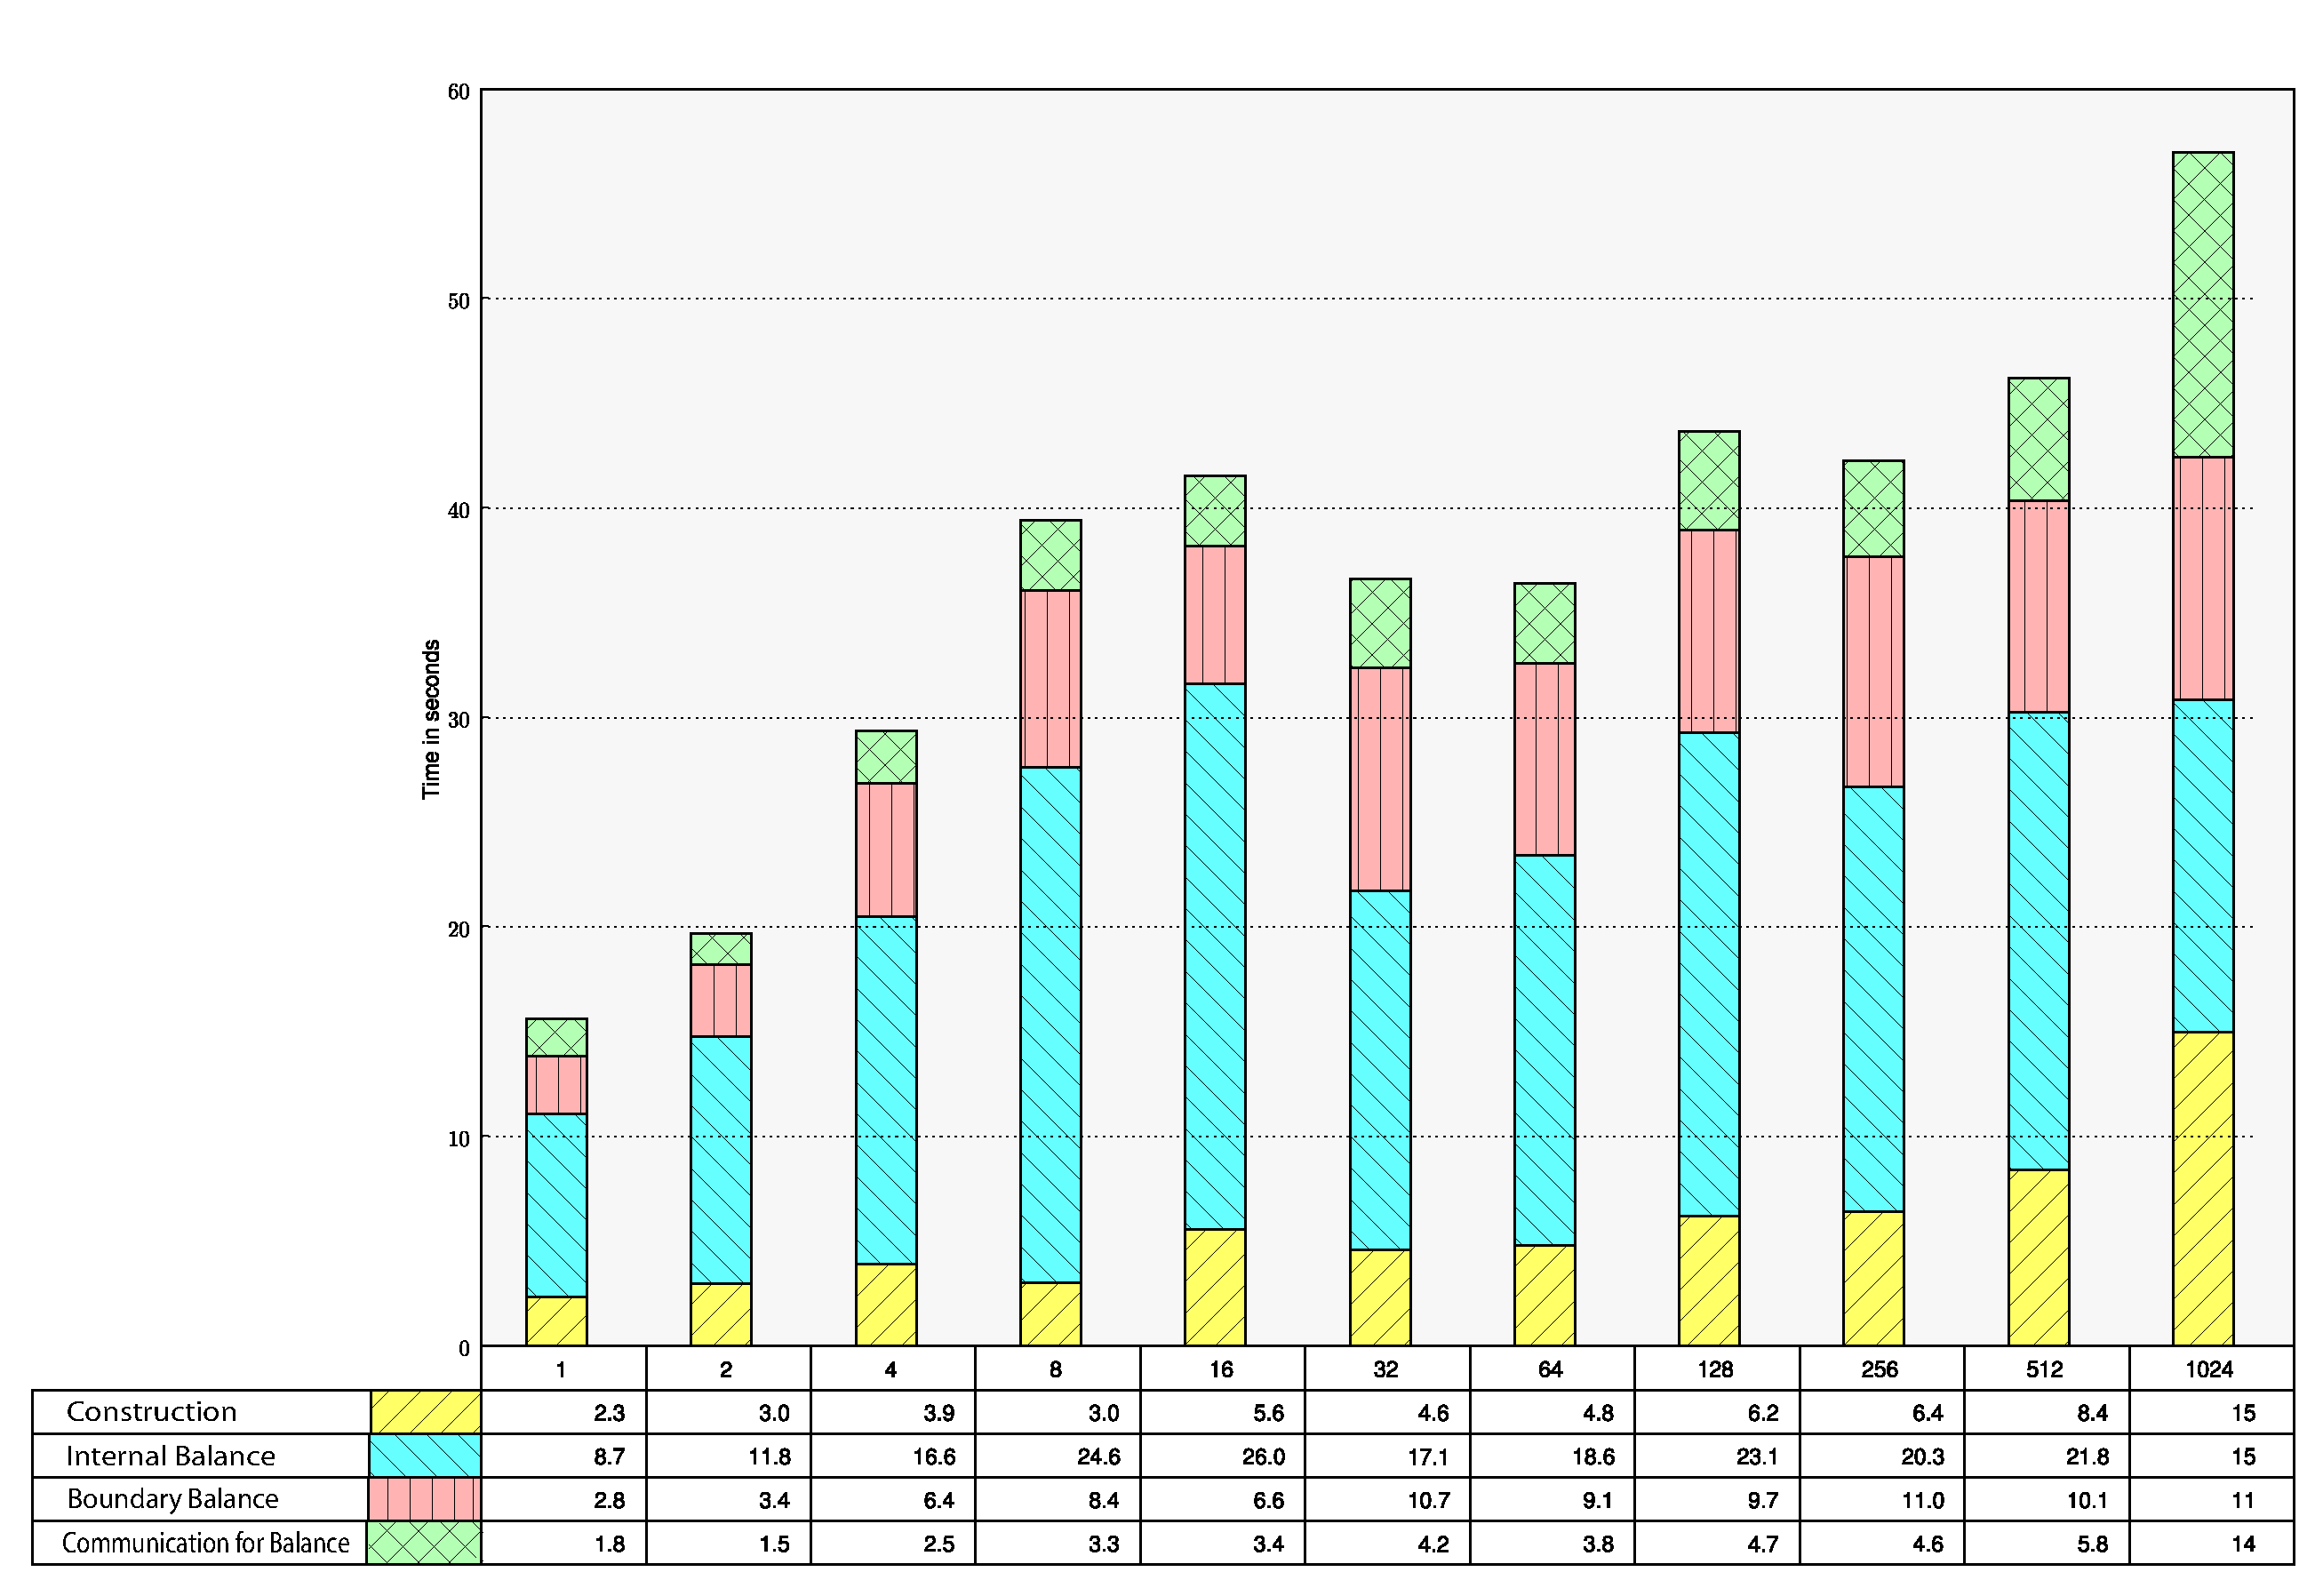
\includegraphics[width=\textwidth]{images/isoGran}
  \end{center}
  \caption{Isogranular scalability for Gaussian distribution of
  {\tt1M} octants per processor. From left to right, the bars indicate
  the time taken for the different components of our algorithms for
  increasing processor counts. The bar for each processor is
  partitioned into {\tt4} sections. From top to bottom, the sections
  represent the time taken for {\tt(1)} communication (including
  related pre-processing and post-processing) during balance
  refinement {\tt(Algorithm \ref{alg:parBal})}, {\tt(2)} balancing
  across intra and inter processor boundaries {\tt(Algorithm
  \ref{alg:ripple})}, {\tt(3)} balancing the blocks {\tt(Algorithm
  \ref{alg:effConBal})} and {\tt(4)} construction from points
  {\tt(Algorithm \ref{alg:p2o})}.}
  \label{fig:isoG}
\end{figure}

\begin{figure}
  \begin{center}
    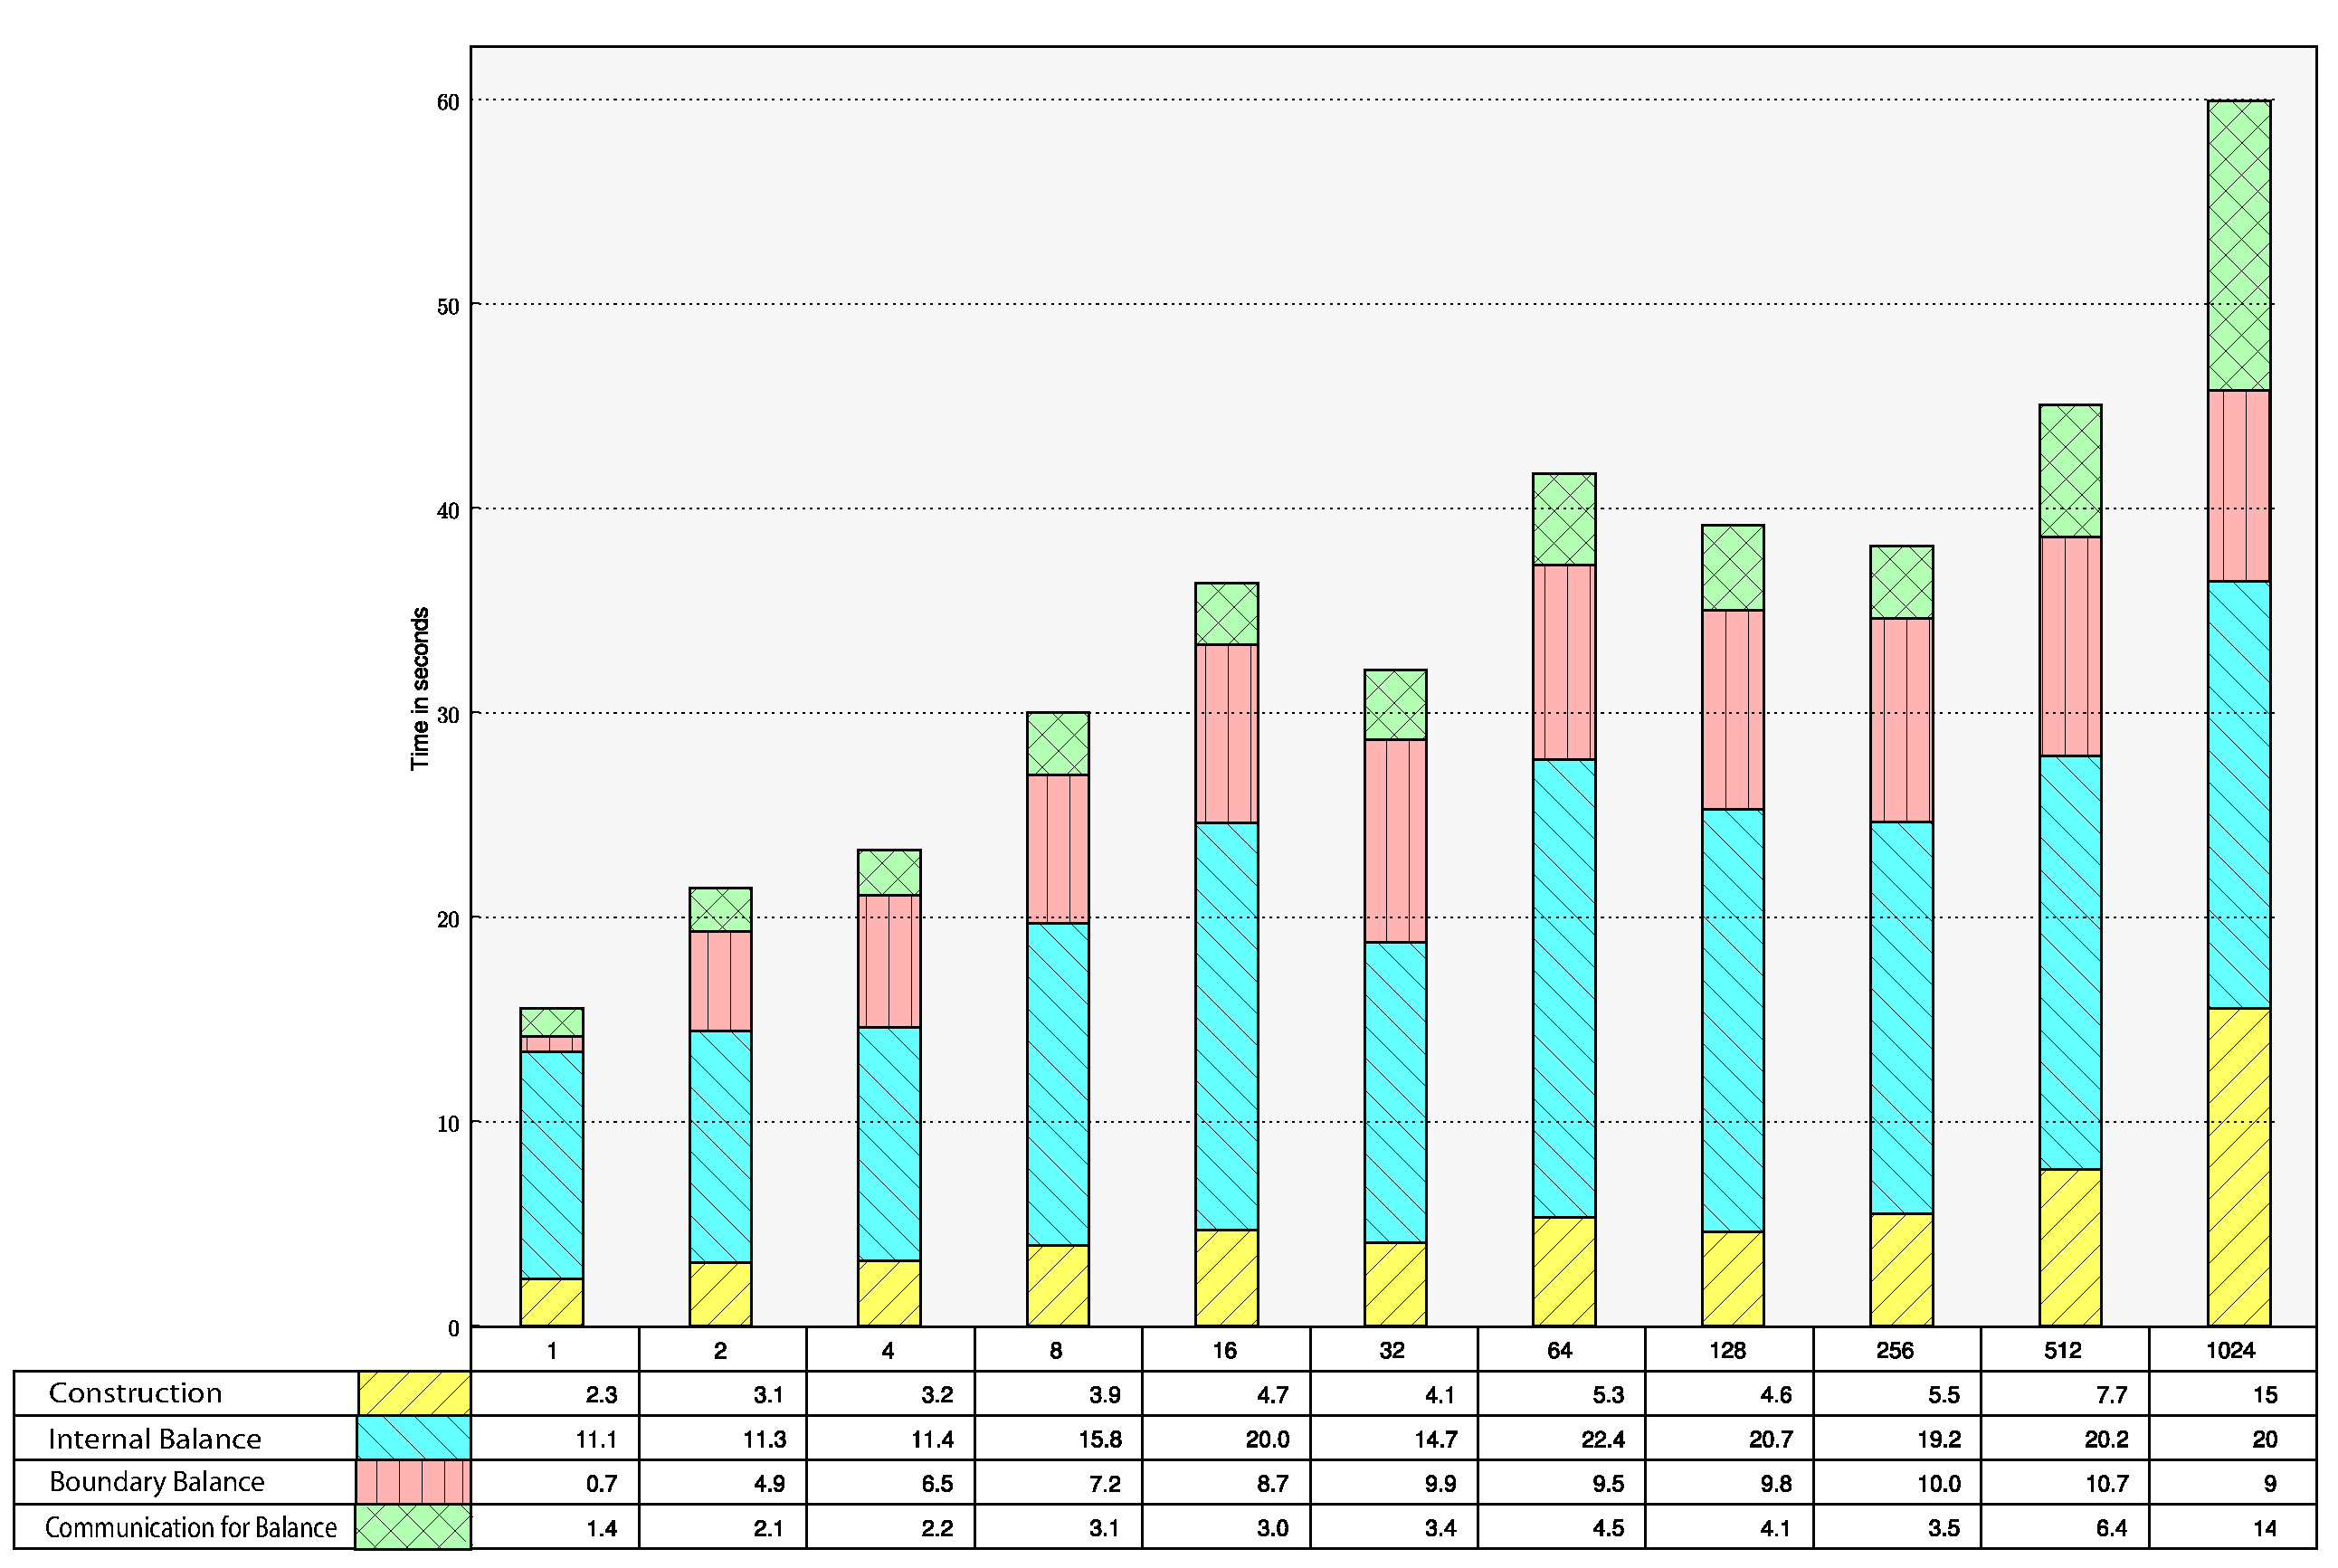
\includegraphics[width=\textwidth]{images/isoLN}
  \end{center}
  \caption{Isogranular scalability for Log-normal distribution of
  {\tt1M} octants per processor. From left to right, the bars indicate
  the time taken for the different components of our algorithms for
  increasing processor counts. The bar for each processor is
  partitioned into {\tt4} sections. From top to bottom, the sections
  represent the time taken for {\tt(1)} communication (including
  related pre-processing and post-processing) during balance
  refinement {\tt(Algorithm \ref{alg:parBal})}, {\tt(2)} balancing
  across intra and inter processor boundaries {\tt(Algorithm
  \ref{alg:ripple})}, {\tt(3)} balancing the blocks {\tt(Algorithm
  \ref{alg:effConBal})} and {\tt(4)} construction from points
  {\tt(Algorithm \ref{alg:p2o})}.}
  \label{fig:isoLN}
\end{figure}

\begin{figure}
  \begin{center}
    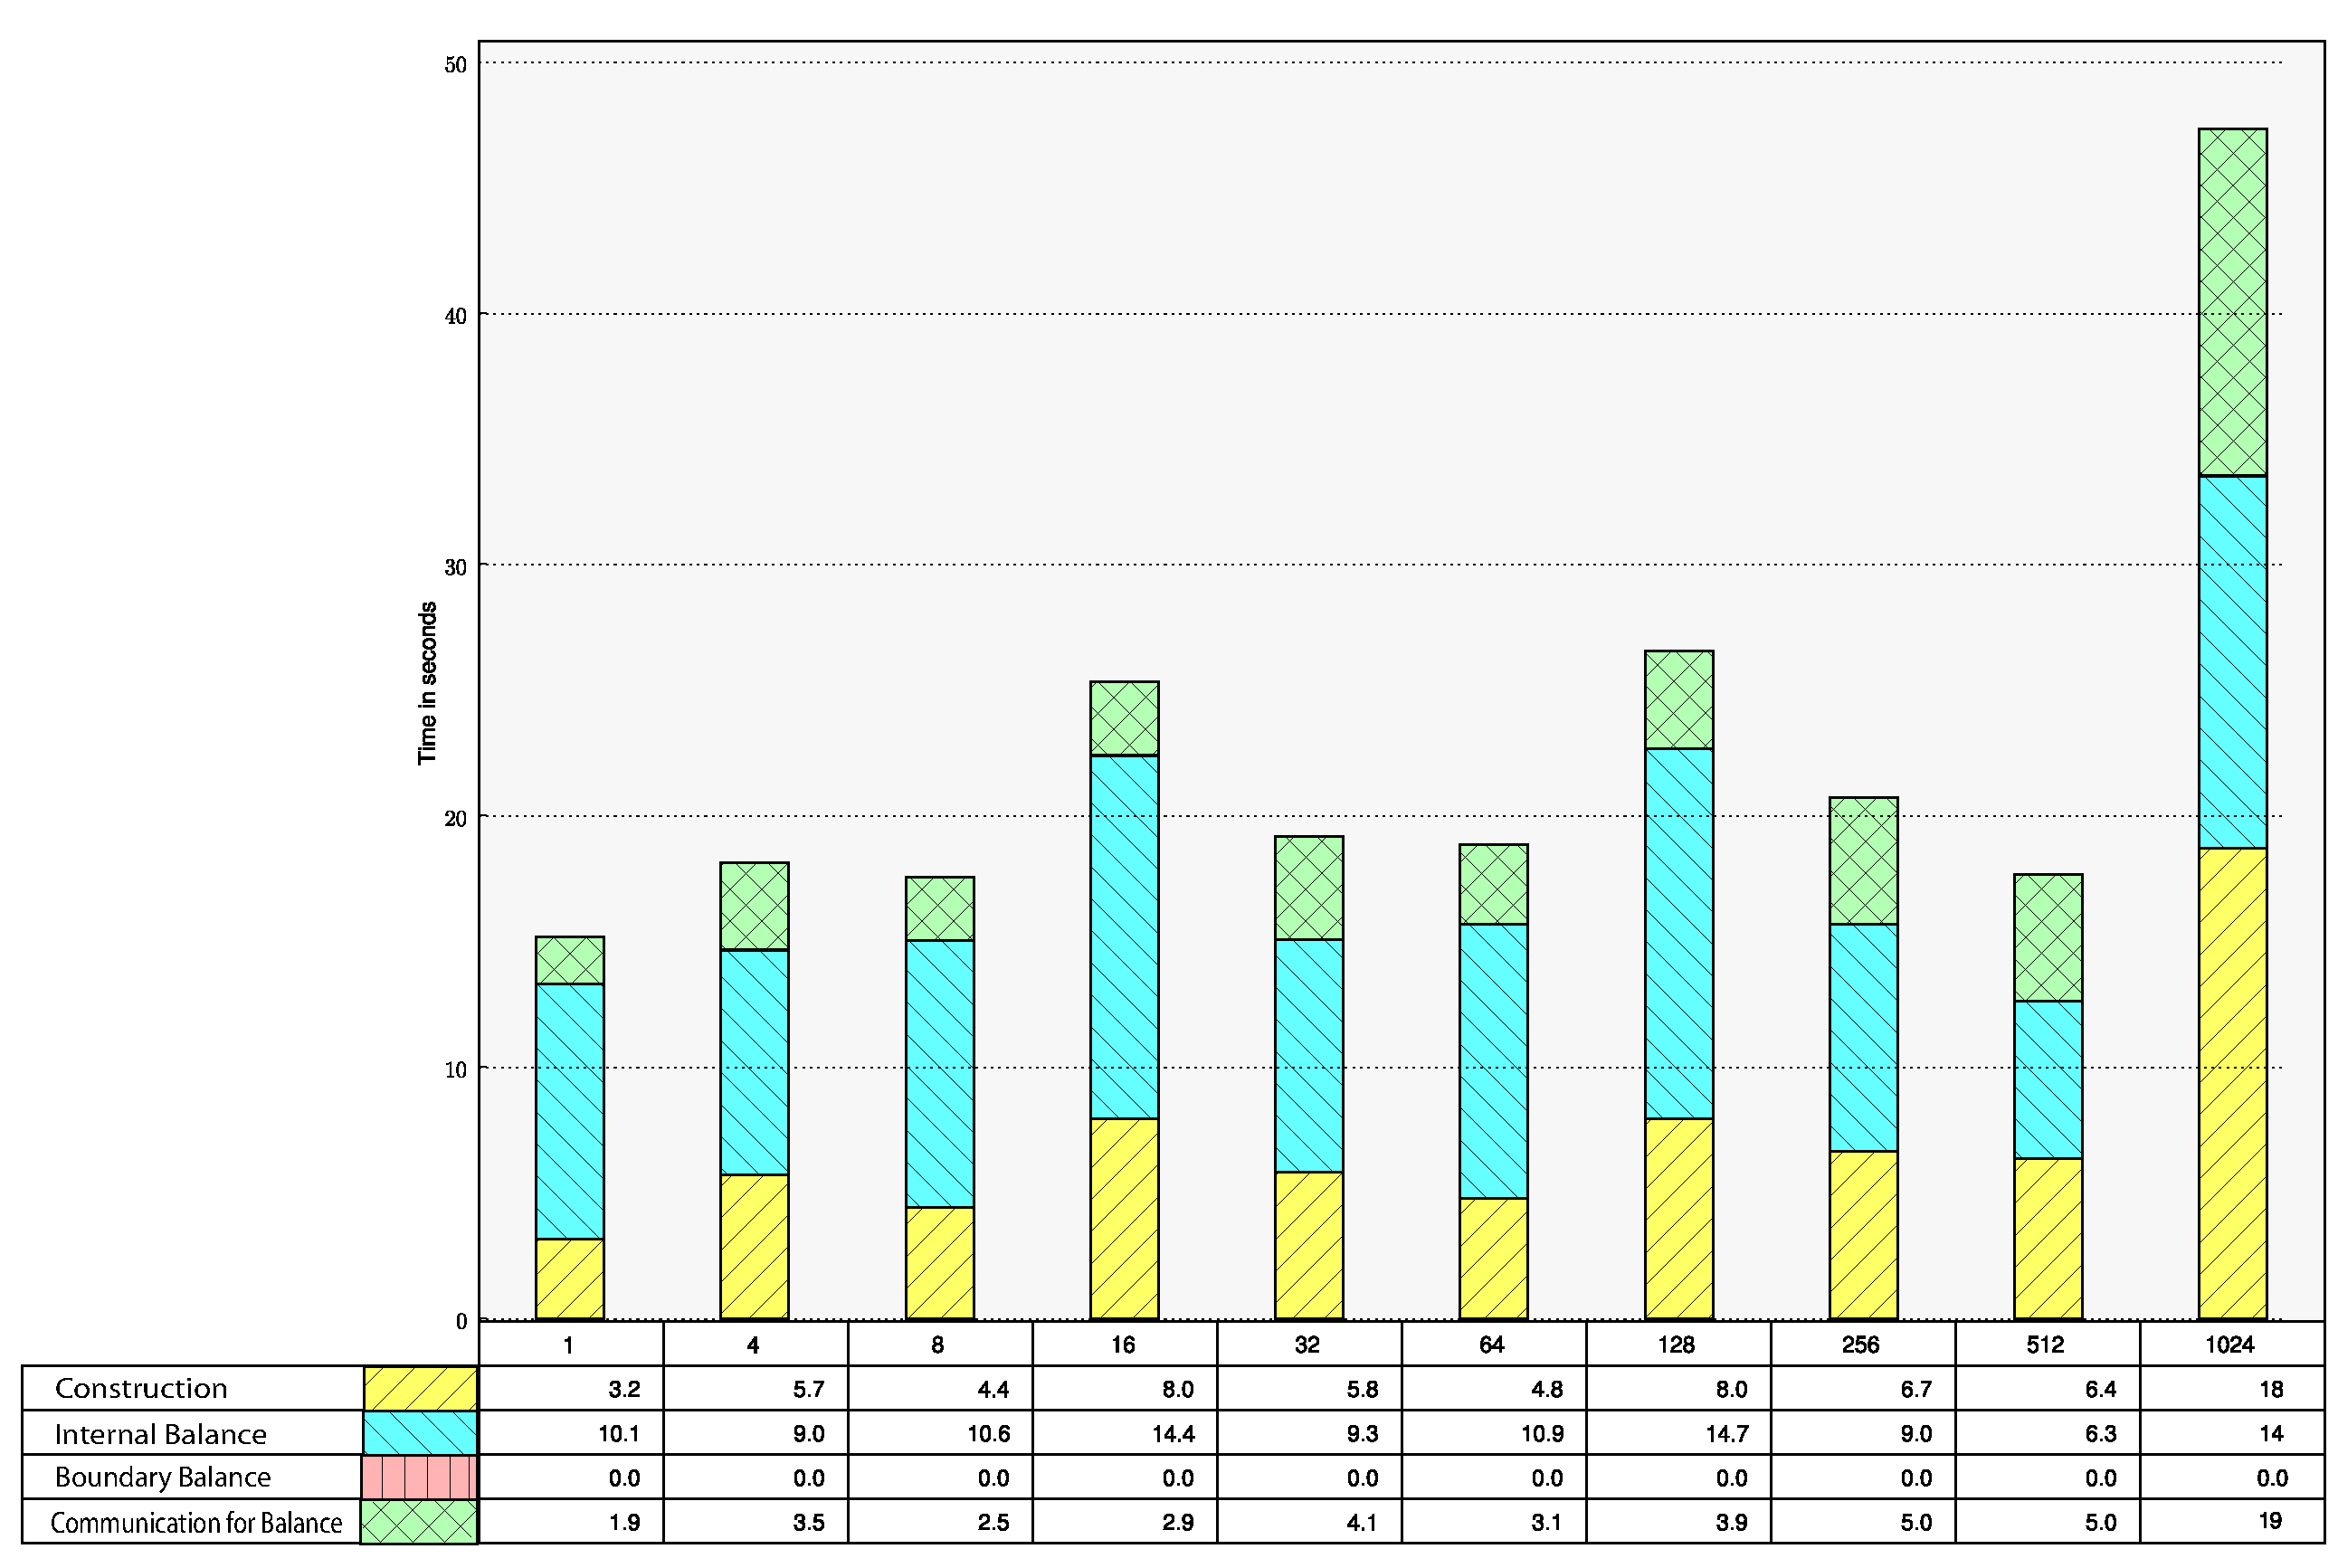
\includegraphics[width=\textwidth]{images/isoRG}
  \end{center}
  \caption{Isogranular scalability for uniformly spaced points with
  {\tt1M} octants per processor. From left to right, the bars indicate
  the time taken for the different components of our algorithms for
  increasing processor counts. The bar for each processor is
  partitioned into {\tt4} sections. From top to bottom, the sections
  represent the time taken for {\tt(1)} communication (including
  related pre-processing and post-processing) during balance
  refinement {\tt(Algorithm \ref{alg:parBal})}, {\tt(2)} balancing
  across intra and inter processor boundaries {\tt(Algorithm
  \ref{alg:ripple})}, {\tt(3)} balancing the blocks {\tt(Algorithm
  \ref{alg:effConBal})} and {\tt(4)} construction from points
  {\tt(Algorithm \ref{alg:p2o})}. While both the input and output
  grain sizes remain almost constant for the Gaussian and LogNormal
  distributions, only the output grain size remains constant for the
  Uniform distribution. Hence, the trend seen in this study is a
  little different from those for the Gaussian and LogNormal
  distributions.}
  \label{fig:isoRG}
\end{figure}

Fixed size scalability tests were also performed for three problem set
sizes, small (1 million points), medium (32 million points) and large
(128 million points), for the Gaussian distribution. These results are
plotted in Figures \ref{fig:fsS}, \ref{fig:fsM} and \ref{fig:fsL}.

\begin{figure}
  \begin{center}
    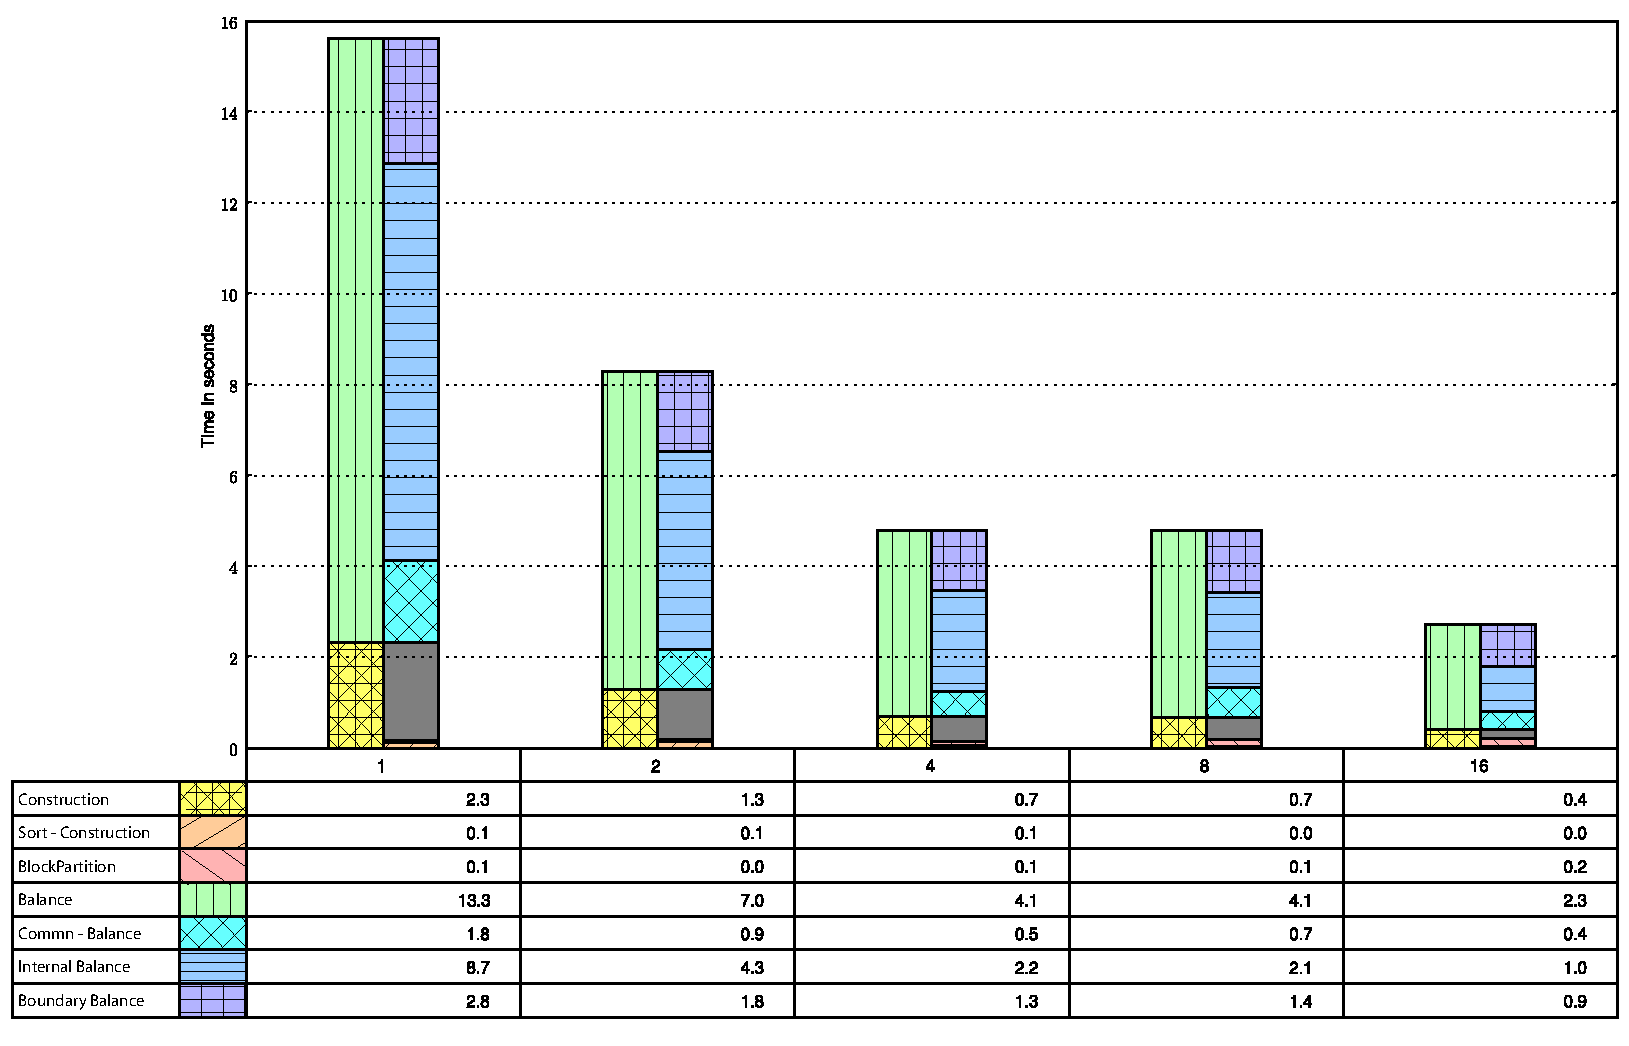
\includegraphics[width=0.9\textwidth]{images/fs1}
  \end{center}
  \caption{Fixed size scalability for Gaussian distribution of {\tt1M}
  octants. From left to right, the bars indicate the time taken for
  the different components of our algorithms for increasing processor
  counts. The bar for each processor is partitioned into {\tt2}
  columns, which are further subdivided. The left column is subdivided
  into {\tt2} sections and the right column is subdivided into {\tt6}
  sections. The top and bottom sections of the left column represent
  the total time taken for {\tt(1)} balance refinement {\tt(Algorithm
  \ref{alg:parBal})} and {\tt(2)} construction {\tt(Algorithm
  \ref{alg:p2o})}, respectively. From top to bottom, the sections of
  the right column represent the time taken for {\tt(1)} balancing
  across intra and inter processor boundaries {\tt(Algorithm
  \ref{alg:ripple})}, {\tt(2)} balancing the blocks {\tt(Algorithm
  \ref{alg:effConBal})}, {\tt(3)} communication (including related
  pre-processing and post-processing) during balance refinement,
  {\tt(4)} local processing during construction, {\tt(5)} {\tt
  BlockPartition} and {\tt(6)} {\tt Sample Sort}.}
  \label{fig:fsS}
\end{figure}

\begin{figure}
  \begin{center}
    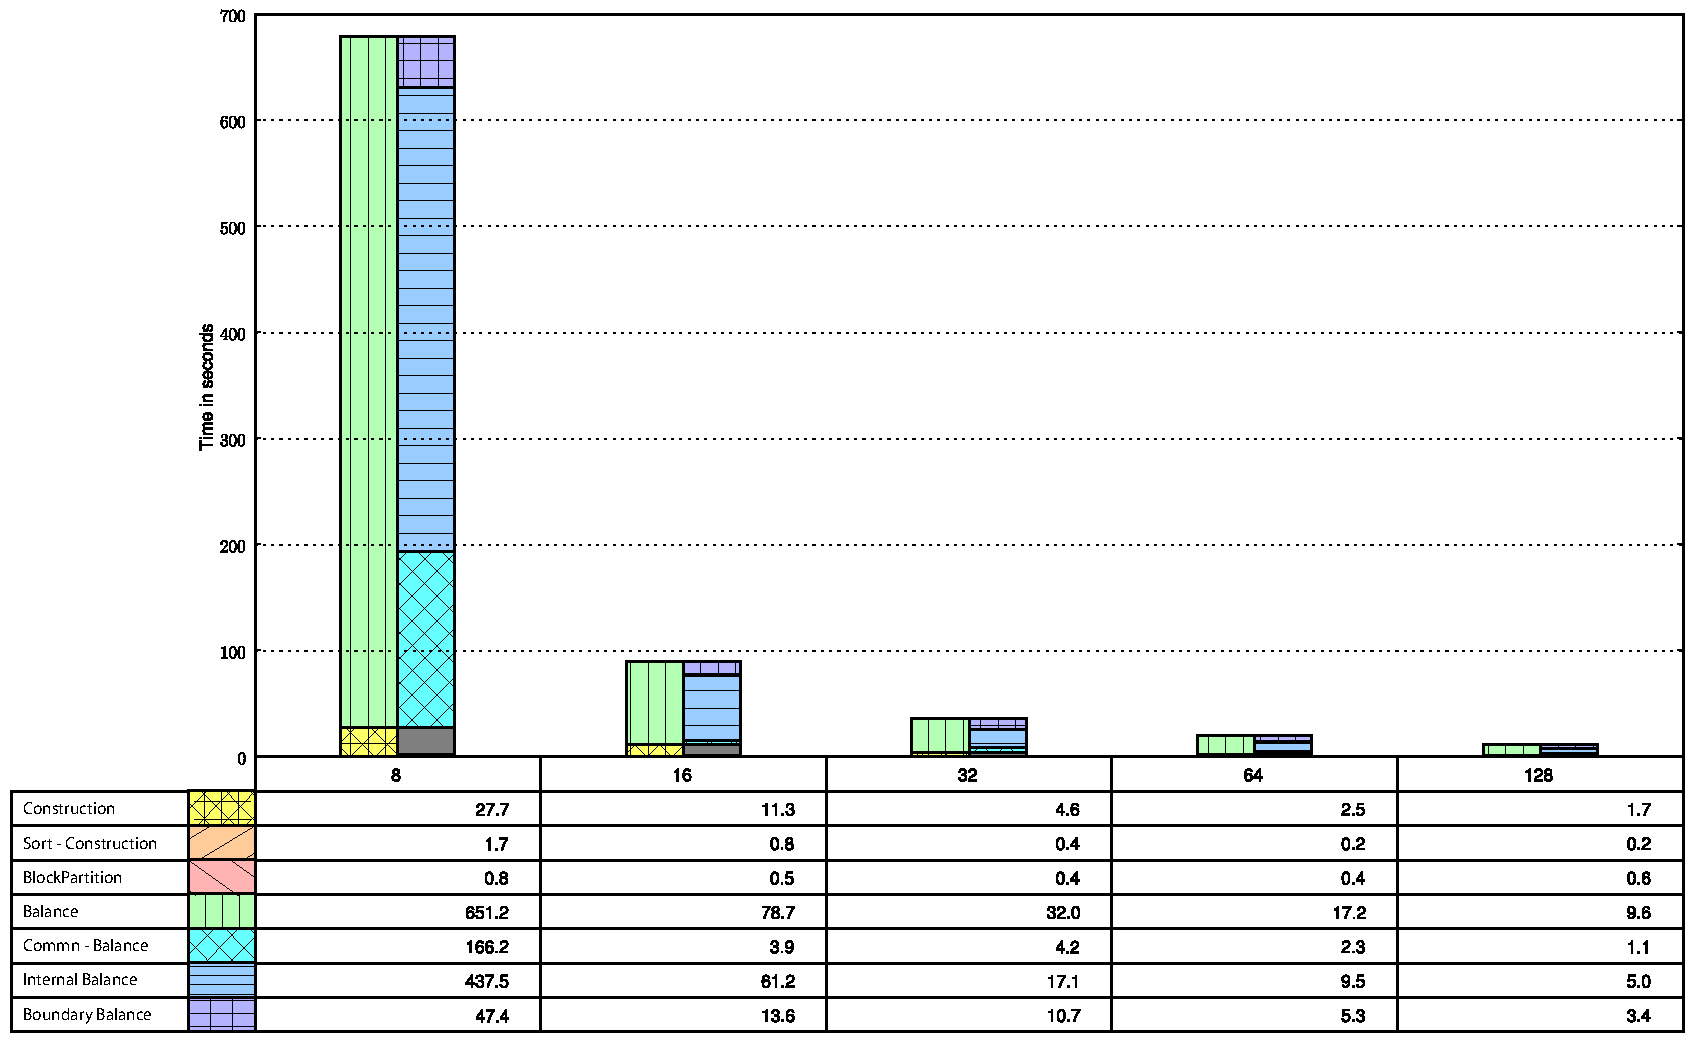
\includegraphics[width=0.9\textwidth]{images/fs32}
  \end{center}
  \caption{Fixed size scalability for Gaussian distribution of
  {\tt32M} octants. From left to right, the bars indicate the time
  taken for the different components of our algorithms for increasing
  processor counts. The bar for each processor is partitioned into
  {\tt2} columns, which are further subdivided. The left column is
  subdivided into {\tt2} sections and the right column is subdivided
  into {\tt6} sections. The top and bottom sections of the left column
  represent the total time taken for {\tt(1)} balance refinement
  {\tt(Algorithm \ref{alg:parBal})} and {\tt(2)} construction
  {\tt(Algorithm \ref{alg:p2o})}, respectively. From top to bottom,
  the sections of the right column represent the time taken for
  {\tt(1)} balancing across intra and inter processor boundaries
  {\tt(Algorithm \ref{alg:ripple})}, {\tt(2)} balancing the blocks
  {\tt(Algorithm \ref{alg:effConBal})}, {\tt(3)} communication
  (including related pre-processing and post-processing) during
  balance refinement, {\tt(4)} local processing during construction,
  {\tt(5)} {\tt BlockPartition} and {\tt(6)} {\tt Sample Sort}.}
  \label{fig:fsM}
\end{figure}

\begin{figure}
  \begin{center}
    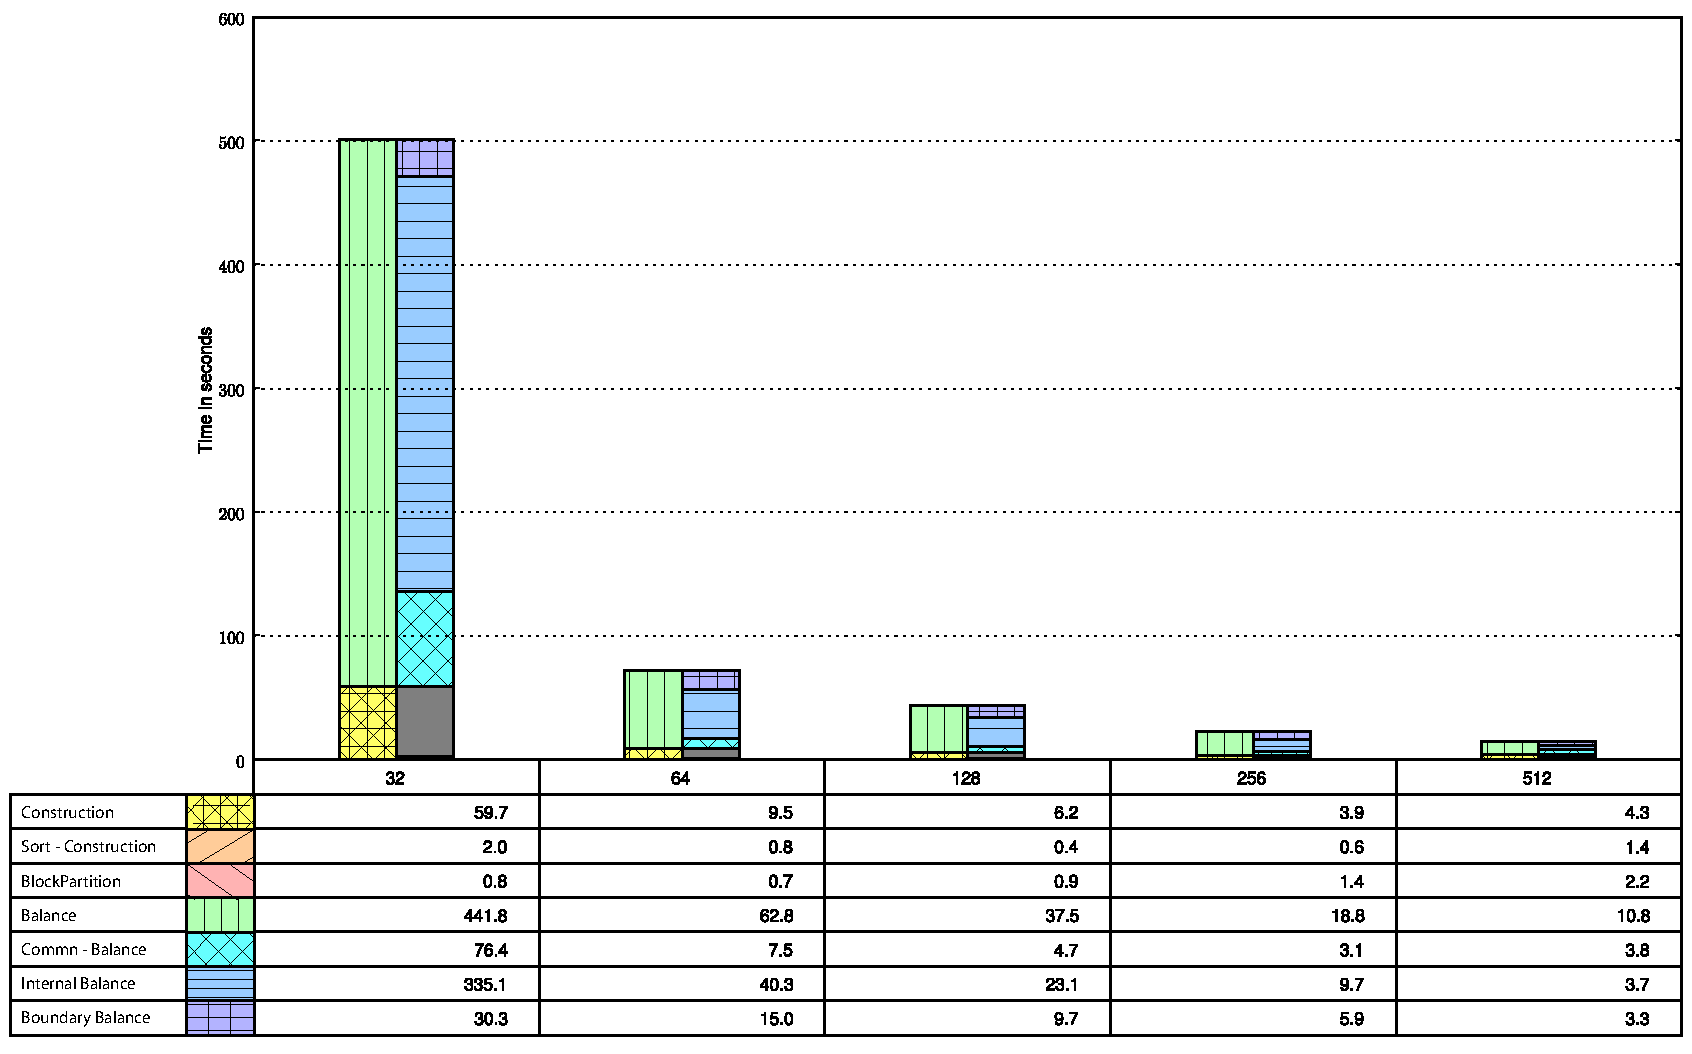
\includegraphics[width=0.9\textwidth]{images/fs128}
  \end{center}
  \caption{Fixed size scalability for Gaussian distribution of
  {\tt128M} octants. From left to right, the bars indicate the time
  taken for the different components of our algorithms for increasing
  processor counts. The bar for each processor is partitioned into
  {\tt2} columns, which are further subdivided. The left column is
  subdivided into {\tt2} sections and the right column is subdivided
  into {\tt6} sections. The top and bottom sections of the left column
  represent the total time taken for {\tt(1)} balance refinement
  {\tt(Algorithm \ref{alg:parBal})} and {\tt(2)} construction
  {\tt(Algorithm \ref{alg:p2o})}, respectively. From top to bottom,
  the sections of the right column represent the time taken for
  {\tt(1)} balancing across intra and inter processor boundaries
  {\tt(Algorithm \ref{alg:ripple})}, {\tt(2)} balancing the blocks
  {\tt(Algorithm \ref{alg:effConBal})}, {\tt(3)} communication
  (including related pre-processing and post-processing) during
  balance refinement, {\tt(4)} local processing during construction,
  {\tt(5)} {\tt BlockPartition} and {\tt(6)} {\tt Sample Sort}.}
  \label{fig:fsL}
\end{figure}

%}}}

%{{{ conclusions
\section{Conclusions}
\label{sec:conclude}
We have presented two new parallel algorithms for constructing and
balancing large linear octrees on distributed memory machines. We have
also tested MPI-based scalable parallel implementations for both the
algorithms.  Our algorithms have several important features:
\begin{itemize}
\item Experiments on three different types of input distributions
demonstrate that the algorithms are insensitive to the underlying data
distribution.
\item Our algorithms avoid iterative communications and thus are able
to achieve low absolute runtime and good scalability.
\item The experiments for comparing the performance of different
algorithms for the local balancing stage demonstrated that the one
proposed in this paper has a significantly lower running time than the
others.
\item We demonstrated scalability up to 1024 processors: we were able
to construct and balance octrees with over 1 billion octants in less
than a minute.
\end{itemize}

We need to consider the following factors to improve the performance
of the proposed algorithms. In order to minimize communication costs,
it is desirable to have as large coarse blocks as possible since the
communication cost is proportional to the area of the inter-processor
boundaries. However, too coarse blocks will increase the work for the
local block balancing stage (Section \ref{sec:conBal}). If additional
local splits are introduced, then the intra-block boundaries increase
causing the work load for the first ripple balance to increase. The
local balancing step of the algorithm can be made more efficient by
performing the local balancing recursively by estimating the correct
size of the block that can be balanced by the search-free
approach. Such an approach should be based on low-level architecture
details, like the cache size. %We intend to further improve the
%performance of our algorithms by adapting the algorithm to minimize
%cache misses.

%{{{ Morton encoding properties
\section{Properties of Morton encoding}
\label{app:prop}

\begin{prop}
Sorting all the leaves in the ascending order of their Morton ids is
identical to a preorder traversal of the leaves of the octree. If one
connects the centers of the leaves in this order, one can observe a
Z-pattern in the Cartesian space. The space-filling Z-order curve has
the property that spatially nearby octants tend to be clustered
together. The octants in Figures \ref{fig:completeOctree} and
\ref{fig:balancedOctree} are all labeled according to this
order. Depending on the order of interleaving the coordinates,
different Z-order curves are obtained. The two possible Z-curves in
2-D are shown in the Figure \ref{fig:ztypes}. Similarly, in 3-D six
different types of Morton ordering are possible.
  \label{ZdefProp}
\end{prop}

\begin{figure}
  \begin{center}
    \includegraphics[width=0.5\textwidth]{images/MortonZtypes}  
  \end{center}
  \caption{Two types of z-ordering in quadtrees.}
    \label{fig:ztypes}
\end{figure}

\begin{prop}
Given three octants, $a < b < c$ and $c \notin \{\mathcal{D}(b)\}$:
  \[
  a < d < c, ~~\forall d \in \{\mathcal{D}(b)\}.
  \]
  \label{prop:decFirst}
\end{prop}

\begin{prop}
The Morton id of any node is less than those of its descendants.
  \label{prop:ancLesser}
\end{prop}

\begin{prop}
Two distinct octants overlap if and only if one is an ancestor of the
other.
\label{prop:overlap}
\end{prop}

\begin{prop}
The Morton id of any node and of its first child\footnote{the child
that has the same anchor as the parent} are consecutive. It follows
from Property \ref{prop:ancLesser} that the first child is also the
child with the least Morton id.
  \label{prop:fcProp}
\end{prop}

\begin{prop}
The first descendant at level $l$, denoted by
$\mathcal{FD}\left(N,l\right)$, of any node $N$ is the descendant at
level $l$ with the least Morton id. This can be arrived at by
following the first child at every level starting from
$N$. $\mathcal{FD}\left(N,D_{max}\right)$ is also the anchor of $N$
and is also referred to as the {\em deepest first descendant}, denoted
by $\mathcal{DFD}(N)$, of node $N$.
  \label{prop:fdProp}
\end{prop}

\begin{prop}
The range $(N,\mathcal{DFD}(N)]$ only contains the first descendants
of $N$ at different levels and hence there can be no more than one
leaf in this range in the entire linear octree.
  \label{prop:rangeFprop}
\end{prop}

\begin{prop}
The {\em last descendant} at level $l$, denoted by
$\mathcal{LD}\left(N,l\right)$, of any node $N$ is the descendant at
level $l$ with the greatest Morton id. This can be arrived at by
following the {\em last child}\footnote{child with the greatest Morton
id} at every level starting from
$N$. $\mathcal{LD}\left(N,D_{max}\right)$ is also referred to as the
{\em deepest last descendant}, denoted by $\mathcal{DLD}(N)$, of node
$N$.
  \label{prop:ldProp}
\end{prop}

\begin{prop}
Every octant in the range $(N,\mathcal{DLD}(N)]$ is a descendant of
$N$.
  \label{prop:rangeLprop}
\end{prop}
%}}}

%{{{ Multicomponent representation
\section{Multicomponent Morton Representation}
\label{app:mortonClass}
Every Morton id is a set of 4 entities: The three co-ordinates of the
anchor of the octant and the level of the octant. We have implemented
the node as a C++ class, which contains these 4 entities as its member
data. To use this set as a locational code for octants, we define two
primary binary logical operations on it: a) Comparing if 2 ids are
equal and b) Comparing if one id is lesser than the other.

Two ids are equal if and only if all the 4 entities are respectively
equal. If two ids have the same anchor then the one at a coarser level
has a lesser Morton id. If the anchors are different, then we can use
Algorithm \ref{alg:lessOp} to determine the lesser id. The Z-ordering
produced by this operator is identical to that produced by the scalar
Morton ids described in section \ref{sec:morton}. The other logical
operations can be readily derived from these two operations.


\begin{table*}
\centering
\rule{\textwidth}{0.01mm}
\begin{algorithm}{ \textsc{Finding the lesser of two Morton ids (sequential)}}
\rule{\textwidth}{0.01mm}
\flushleft
\tt{\bf{Input:~} Two Morton ids, $A$ and $B$ with different anchors.} \\
\tt{\bf{Output:} $R,$ the lesser of the two Morton ids.}\\
~\\
1. $X_i \leftarrow \left(A_i \oplus B_i\right)$, $i \in \{x, y, z\}$\\
2. $e \leftarrow \argmax{i} (\lfloor\log_2(X_i)\rfloor)$ \\
\begin{tabbing}
3. {\bf if} \= $A_e < B_e$ \\
           \> $R \leftarrow A$\\
4. {\bf else} \\
             \>  $R \leftarrow B$\\
5. {\bf end if}
\end{tabbing}
\label{alg:lessOp}
\end{algorithm}
\rule{\textwidth}{0.01mm}
\end{table*}
%}}}

%{{{ Block partitionings
\section{Analysis of the Block Partitioning Algorithm}
\label{app:blkPartAnal}
Assume that the input to the partitioning algorithm is a sorted
distributed list of $N$ octants. Then, we can guarantee coarsening of
the input if there are more than {\tt8} octants\footnote{$2^d$ cells
for a $d$-tree.} per processor. The minimum number of octants on any
processor, $n_{min},$ can be expressed in terms of $N$ and the
imbalance factor\footnote{The imbalance factor is the ratio between
the maximum and minimum number of octants on any processor.}, $c,$ as
follows:
\[
n_{min} = \frac{N}{1+c(n_p-1)}.
\]

This implies that the coarsening algorithm will coarsen the octree if,
\begin{eqnarray*}
n_{min} = \frac{N}{1+c(n_p-1)} & > & 2^d, \\
\implies N > 2^d(1 + c(n_p - 1)).
\end{eqnarray*}

The total number of blocks created by our coarsening algorithm is
$\mathcal{O}(p)$. Specifically, the total number of blocks produced by
the coarsening algorithm, $N_{blocks}$, satisfies:
\[
p \le N_{blocks} < 2^d p.
\]

If the input is sorted and if $c \approx 1$, then the communication
cost for this partition is $\mathcal{O}(\frac{N}{n_p})$.
%}}}

%{{{ Special case while constructiong
\section{Special case during construction}
\label{app:specialCon}
We can not always guarantee the coarsest possible octree for an
arbitrary distribution of $N$ points and arbitrary values of
$N^p_{max}$, especially when $N^p_{max} \approx
\frac{N}{n_p}$. However, if every processor has at least 2
{\em{well-separated}} \footnote{Convert the points into octants at
$D_{max}$ level. If there exists at least one coarse octant between
these two octants, then the points are considered to be
well-separated.} points and if $N^p_{max}=1$, then the algorithm will
produce the coarsest possible octree under these constraints.
However, this is not too restrictive because the input points can
always be sampled in such a way that the algorithm produces the
desired octree. Besides, the maximum depth of the octree can also be
used to control the coarseness of the resulting octree. In all our
experiments, we used $N^p_{max}=1$ and we always got the same octree
for different number of processor counts (Table \ref{tab:numbers}).
%}}}

